\documentclass[12pt,a4paper]{report}
\usepackage{amsmath,amssymb}
\usepackage[hidelinks]{hyperref}
\usepackage{algorithm}
\usepackage{algorithmic}
\usepackage{graphicx}
\usepackage{subcaption}
\usepackage{times}
\usepackage{multirow}
\usepackage{float}
\usepackage{setspace}
\usepackage{booktabs}
\usepackage{titlesec}
\usepackage[backend=biber,style=numeric,citestyle=numeric]{biblatex}
\addbibresource{references.bib}

\titleformat{\chapter}[display]
    {\normalfont\bfseries\raggedright}
    {\fontsize{18}{18}\selectfont Chapter \thechapter}
    {15pt}
    {\fontsize{18}{18}\selectfont}

\titlespacing*{\chapter}
    {0pt}{-80pt}{20pt}

\titleformat{\section}
    {\normalfont\bfseries\fontsize{16}{16}\selectfont}
    {\thesection}
    {0.5cm}
    {}

\titlespacing*{\section}
    {0pt}{15pt}{10pt}
    
\begin{document}
\pagenumbering{roman}
\begin{titlepage}
\begin{center}
\vspace*{0.3cm}
{\fontsize{24}{28}\selectfont\bfseries
Score Matching techniques on Goodness of-Fit tests
}

\vspace{0.5cm}
{\fontsize{14}{17}\selectfont
An internship report for partial fulfillment of the
requirements for the Degree of
}

\vspace{0.5cm}
{\fontsize{20}{24}\selectfont\bfseries
Master of Technology
}

\vspace{0.3cm}
{\fontsize{14}{17}\selectfont
in
}

\vspace{0.3cm}
{\fontsize{16}{19}\selectfont\bfseries
Communication and Signal Processing
}

\vspace{0.5cm}
{\fontsize{14}{17}\selectfont
by
}

\vspace{0.3cm}
{\fontsize{14}{146}\selectfont\bfseries
Dibyanshu Shekhar Dey
}

\vspace{0.3cm}
{\fontsize{14}{17}\selectfont
Under the guidance of 
}

\vspace{0.3cm}
{\fontsize{14}{146}\selectfont\bfseries
Prof. Subhadip Mukherjee
}


\vspace{1.5cm}

\includegraphics[width=3.2cm]{report_images/iitkgplogo.jpg}
\vfill

{\fontsize{13}{16}\selectfont
Department of Electronics and Electrical Communication Engineering
}

\vspace{0.2cm}

{\fontsize{16}{19}\selectfont\bfseries
INDIAN INSTITUTE OF TECHNOLOGY KHARAGPUR
}

\vspace{0.2cm}

{\fontsize{13}{16}\selectfont
Kharagpur - 721302
}

\vspace{0.8cm}

{\fontsize{14}{17}\selectfont
September 2026
}
\end{center}
\end{titlepage}

% Table of Contents
\tableofcontents
\newpage

% Abstract
\chapter*{Abstract}
\addcontentsline{toc}{chapter}{Abstract}
\vspace{0.3cm}
\noindent
The problem of checking if a sample comes from a known distribution is already well established. For images, real life application involves CT scans, X-rays and more recently generative images. It becomes important to spot the out of distribution (OOD) images especially if the irregular information in images might be too minute, which makes the detection of OOD images quite difficult.

\vspace{0.3cm}
\noindent
This work tries to go in the direction of addressing these problem. First we use a test statistic, called Kernelized Stein Discrepancy (KSD) that utilizes the score functions to address the hypothesis test. However real life datasets do not involve well defined distributions, which makes the use of score function seemingly impossible. We then utilize another metric - Score Matching, which makes use of the U-Net architecture for image datasets to learn the score function and then we plug-in this learned function into our KSD framework, and do the test all over again.

\vspace{0.3cm}
\noindent
We then use diffusion posterior sampling which uses the learned score to generate a new set of samples from the test dataset. We then employ the KSD statistic on these generated image dataset to detect the statistical power, and also check quality of these images using PSNR and SSIM curves.

\vspace{0.3cm}
\noindent
The code of this report can be found on this link
\url{https://github.com/dibyanshushekhardey/Summer_Research_Intern_2026}.

% chapter 1 introduction
\clearpage

\pagenumbering{arabic}
\setcounter{page}{1}
\chapter{Introduction}
\section{Background}
Kernelized Stein discrepancy is a powerful test statistic that only requires the samples from the unknown dataset and a score function that is based on in-distribution (InD), to maximize the discriminative power between InD and out-of-distribution (OOD). But for images, we require a trained score network to learn the score of the InD samples. Score matching addresses this problem \cite{song2021scorebasedgenerativemodelingstochastic}. We then combine these two separate metrics into our work.

\section{Motivation}
Goodness-of-Fit test based literature already many such methods - KSD, MMD, Kolmogorov-Smirnov, Chi-Square, Cramer-von-Mises etc. However most of these tests in statistical field are applied for low dimensional datasets. It becomes important to check their application on multidimensional datasets. KSD tests based on U-statistics already perform substantially well that other tests on toy experiments (eg. 1D Gaussian) \cite{liu2016kernelizedsteindiscrepancygoodnessoffit}. Our motivation simply comes to apply this on multidimensional test setting - images, and analyze them. This leads to score matching which give a method to be combined for multidimensional setting in KSD-U framework.

\vspace{0.3cm}
\noindent
This work goes like this: first we use the KSD-U Statistic on toy examples, then train a score model based on image dataset (MNIST) and then design an experiment that utilizes both these techniques.

\vspace{0.3cm}
\noindent
Generative samples can also be tested in our work \cite{chung2024diffusionposteriorsamplinggeneral}. We utilize the diffusion posterior sampling to generate new samples using the motivation from the score matching and then use KSD-U framework on them.

\section{Objectives}

\begin{enumerate}
    \item Develop the KSD-U framework on toy examples.
    \item Perform various perturbation based tests on toy examples.
    \item Train a score function on the MNIST image dataset.
    \item Perform KSD-U on the MNIST dataset.
    \item Generate new samples from MNIST dataset and check the quality of such images.
    \item Take the best quality images and perform the power of the test on the generated images.
\end{enumerate}

% chapter 2 introduction
\chapter{Kernelized Stein Discrepancy}
\section{Preliminary}
A goodness-of-fit test is posed like this - we have two distributions $p(x)$ and $q(x)$, are they same distribution or are they different. Realistic scenarios involve having samples from these two unknown distributions. Two samples tests like MMD involve checking whether two samples come from same distribution or not. However KSD is one sample test. We have samples  $x_i \sim p(x)$ where $p(x)$ is unknown. We have score function $s_q(x) = \nabla_{x} \log q_(x)$ of another distribution $q(x)$. This will be either analytical if $q(x)$ is tractable and we will put the samples from $p(x)$ on this score function or trained on samples from $q(x)$ and then use $p(x)$ samples on the trained score.

\section{Definitions}
The Kernelized Stein discrepancy (KSD) 
$\mathbb{S}(p,q)$ between distribution $p$ and $q$ is defined as
\begin{equation}
    \mathbb{S}(p,q)
    =
    \mathbb{E}_{x,x'\sim p}
    \left[
        \delta_{q,p}(x)^\top
        k(x,x')
        \delta_{q,p}(x')
    \right]
\end{equation}
\noindent
where $\delta_{q,p}(x) = s_q(x)-s_p(x)$ is the score difference between $p$ and $q$, and $x,x'$ are i.i.d. draws from $p(x)$.

\vspace{0.3cm}
\noindent
However we use a KSD estimate if we have the samples from $p(x)$. We use Theorem 3.6 \cite{liu2016kernelizedsteindiscrepancygoodnessoffit} to define the function
\begin{equation}
\begin{aligned}
u_q(x,x')
=
s_q(x)^\top k(x,x')s_q(x')
+ s_q(x)^\top \nabla_{x'} k(x,x') \\
+ \nabla_x k(x,x')^\top s_q(x')
+ \operatorname{trace}\left(\nabla_{x,x'} k(x,x')\right)
\end{aligned}
\label{eq:u_q}
\end{equation}

\noindent
The kernel $k({x},{x}')$ can be any suitable positive
definite kernel. Here, we use the RBF kernel:
\begin{equation}
k({x},{x}')
=
\exp\left(
-\frac{\|{x}-{x}'\|^2}
{2h^2}
\right),
\end{equation}

\noindent
where $h$ is the bandwidth parameter. In particular, we use
\begin{equation}
    h = \sqrt{\frac{D}{2}}.
\end{equation}

\noindent
The bandwidth can also be selected using a median heuristic \cite{garreau2018largesampleanalysismedian}
\begin{equation}
    {D} =
    \operatorname{median}
    \left\{
        \|{x}_i-{x}_j\|
    \right\}_{i\neq j}.
\end{equation}

\section{KSD-U Statistic}
Now the KSD-U uses the U-statistic approach to estimate KSD which is given as 

\begin{equation}
\widehat{\mathbb{S}}_u(p,q)
=
\frac{1}{n(n-1)}
\sum_{1\leq i\neq j\leq n}
u_q(x_i,x_j).
\end{equation}

\noindent
However, to perform the hypothesis test,
we use the bootstrap estimation

\begin{equation}
\widehat{\mathbb{S}}_u^*(p,q)
=
\sum_{i\neq j}
\left(w_i-\frac{1}{n}\right)
\left(w_j-\frac{1}{n}\right)
u_q(x_i,x_j),
\label{eq:ksd_boot}
\end{equation}

\noindent
with
\begin{equation}
(w_1,\ldots,w_n)
\sim
\operatorname{Mult}
\left(
n;\frac{1}{n},\ldots,\frac{1}{n}
\right),
\end{equation}

\noindent
where $w_1,\ldots,w_n$ are multinomial weights.

\section{KSD Goodness-of-Fit Algorithm}
\begin{algorithm}
\caption{KSD-U bootstrap Goodness-of-fit test\cite{liu2016kernelizedsteindiscrepancygoodnessoffit}}

\textbf{Input:} Sample $\{x_i\}$ and score function
$s_q(x) = \nabla_x \log q(x)$. Bootstrap sample size $m$.

\textbf{Test:} $H_0$: $\{x_i\}$ is drawn from $q$ vs.
$H_1$: $\{x_i\}$ is drawn from $p$.

\begin{algorithmic}[1]

\STATE Compute $\widehat{\mathbb{S}}_u$ by  and
$u_q(x,x')$ as defined in Eq.~\eqref{eq:u_q}.
Generate $m$ bootstrap samples $\widehat{\mathbb{S}}_u^*$
by Eq.~\eqref{eq:ksd_boot}.

\STATE Reject $H_0$ with significance level $\alpha$ if the
percentage of $\widehat{\mathbb{S}}_u^*$ that satisfies
\[
\widehat{\mathbb{S}}_u^* > \widehat{\mathbb{S}}_u
\]
is less than $\alpha$.
\end{algorithmic}
\end{algorithm}

\section{Experiments}
Consider the hypotheses $H_0:X\sim\mathcal{N}(0,\sigma^2)$ vs $H_1:X\sim\mathcal{N}(1,\sigma^2)$. We calculate the AUC score. For the single-mode setup, we consider 
\begin{enumerate}
    \item different means that vary according to $\delta \in \{0,\,0.2,\,0.4,\,0.6,\,0.8,\,1.0\}$ keeping $\sigma$ same as $1.0$ for alternate.
    \item different variances $\sigma \in \{0.5,\,0.75,\, 1.0,\, 1.25,\, 1.5, 2.0\}$ keeping the alternate mean fixed as same as null.
\end{enumerate}.

\vspace{0.3cm}
\noindent
We repeat the different means and variances for a different numbers of trials. The AUC is then calculated for the corresponding hypothesis tests with their corresponding ROC curves plotted along with the error rates.

\vspace{0.3cm}
\noindent
We find that the KSD test is able to distinguish between the two distributions very well even when we vary the means and the sigmas, except when it is null. The error rates also decreases significantly if we take sufficient number of samples and perform the tests.

\begin{table}[ht]
    \centering
    \caption{AUC Curves for Single Mode Gaussian Distributions}
    \label{tab:normalized_mse}
    
    \begin{tabular}{c|c|c|c}
        \hline
        Deltas $\delta$ (fixed variance = $1$) & AUC & Sigmas  $\sigma$ (fixed mean = $0$) & AUC \\
        \hline
        $0$  & $0.516$ & $0.5$ & $0.995$ \\ 
        $0.2$  & $0.983$ & $0.75$ & $0.995$ \\
        $0.4$  & $1.0$ & $1.0$ & $0.4828$ \\
        $0.6$  & $0.985$ & $1.25$ & $0.995$ \\
        $0.8$  & $0.975$ & $1.5$ & $0.990$ \\
        $1.0$  & $1.0$ & $1.75$ & $0.985$ \\
        \hline
    \end{tabular}
\end{table}

\begin{table}[ht]
    \centering
    \caption{Error rate for different sample sizes and values of $\delta$.}
    \label{tab:error_delta}

    \begin{tabular}{c|ccccc}
        \hline
        \textbf{Number of samples}
        & $\boldsymbol{\delta=0.25}$
        & $\boldsymbol{\delta=0.5}$
        & $\boldsymbol{\delta=0.75}$
        & $\boldsymbol{\delta=1.0}$
        & $\boldsymbol{\delta=1.5}$ \\
        \hline

        25   & 0.475 & 0.370 & 0.200 & 0.060 & 0.030 \\
        50   & 0.485 & 0.245 & 0.050 & 0.035 & 0.030 \\
        75   & 0.400 & 0.110 & 0.025 & 0.035 & 0.030 \\
        100  & 0.360 & 0.090 & 0.040 & 0.020 & 0.025 \\
        150  & 0.300 & 0.030 & 0.040 & 0.040 & 0.020 \\
        200  & 0.205 & 0.025 & 0.025 & 0.045 & 0.035 \\
        300  & 0.130 & 0.025 & 0.020 & 0.020 & 0.020 \\
        500  & 0.035 & 0.025 & 0.025 & 0.040 & 0.025 \\
        750  & 0.020 & 0.035 & 0.015 & 0.025 & 0.020 \\
        1000 & 0.020 & 0.035 & 0.040 & 0.020 & 0.030 \\

        \hline
    \end{tabular}
\end{table}

\begin{table}[H]
    \centering
    \makebox[\textwidth][c]{%
        \begin{tabular}{c|cccccc}
            \hline
            \textbf{Number of samples}
            & $\boldsymbol{\sigma=0.5}$
            & $\boldsymbol{\sigma=0.75}$
            & $\boldsymbol{\sigma=1.0}$
            & $\boldsymbol{\sigma=1.25}$
            & $\boldsymbol{\sigma=1.5}$
            & $\boldsymbol{\sigma=2.0}$ \\
            \hline

            25   & 0.405 & 0.475 & 0.510 & 0.450 & 0.310 & 0.145 \\
            50   & 0.095 & 0.460 & 0.505 & 0.400 & 0.185 & 0.030 \\
            75   & 0.025 & 0.420 & 0.505 & 0.375 & 0.055 & 0.030 \\
            100  & 0.010 & 0.345 & 0.500 & 0.305 & 0.050 & 0.015 \\
            150  & 0.020 & 0.195 & 0.475 & 0.215 & 0.030 & 0.030 \\
            200  & 0.040 & 0.115 & 0.540 & 0.115 & 0.015 & 0.020 \\
            300  & 0.020 & 0.055 & 0.490 & 0.055 & 0.035 & 0.035 \\
            500  & 0.025 & 0.035 & 0.485 & 0.030 & 0.025 & 0.020 \\
            750  & 0.035 & 0.015 & 0.490 & 0.005 & 0.040 & 0.020 \\
            1000 & 0.035 & 0.025 & 0.510 & 0.030 & 0.015 & 0.035 \\

            \hline
        \end{tabular}%
    }

    \caption{Error rate for different sample sizes and values of $\sigma$.}
    \label{tab:error_delta_sigma}
\end{table}

\section{Discussion}
We went through the toy example setting and used different perturbation techniques on single mode Gaussian mixture model. However, even for this case, the number of samples being taken is very high for the error rate to reduce. Also, this is quite a simple experiment, having to distinguish between two single mode distributions. The future experiments have involve multi modal GMM in which the standard KSD fails \cite{liu2023usingperturbationimprovegoodnessoffit}. We then have used the motivation from this paper and have used different noise scales to perturb the samples and perform the \textbf{Pooled KSD} . This is an ongoing experiment.

\vspace{0.3cm}
\noindent
We also have used standard RBF Kernel, which is a fixed kernel, and does not improve upon the statistical power of the test for multidimensional setting. We are currently working upon this so that this kernel also becomes a learned kernel. We have not performed the tests using standard IMQ kernel.

\begin{figure}[htbp]
    \centering
    % First row
    \begin{subfigure}{0.45\textwidth}
        \centering
        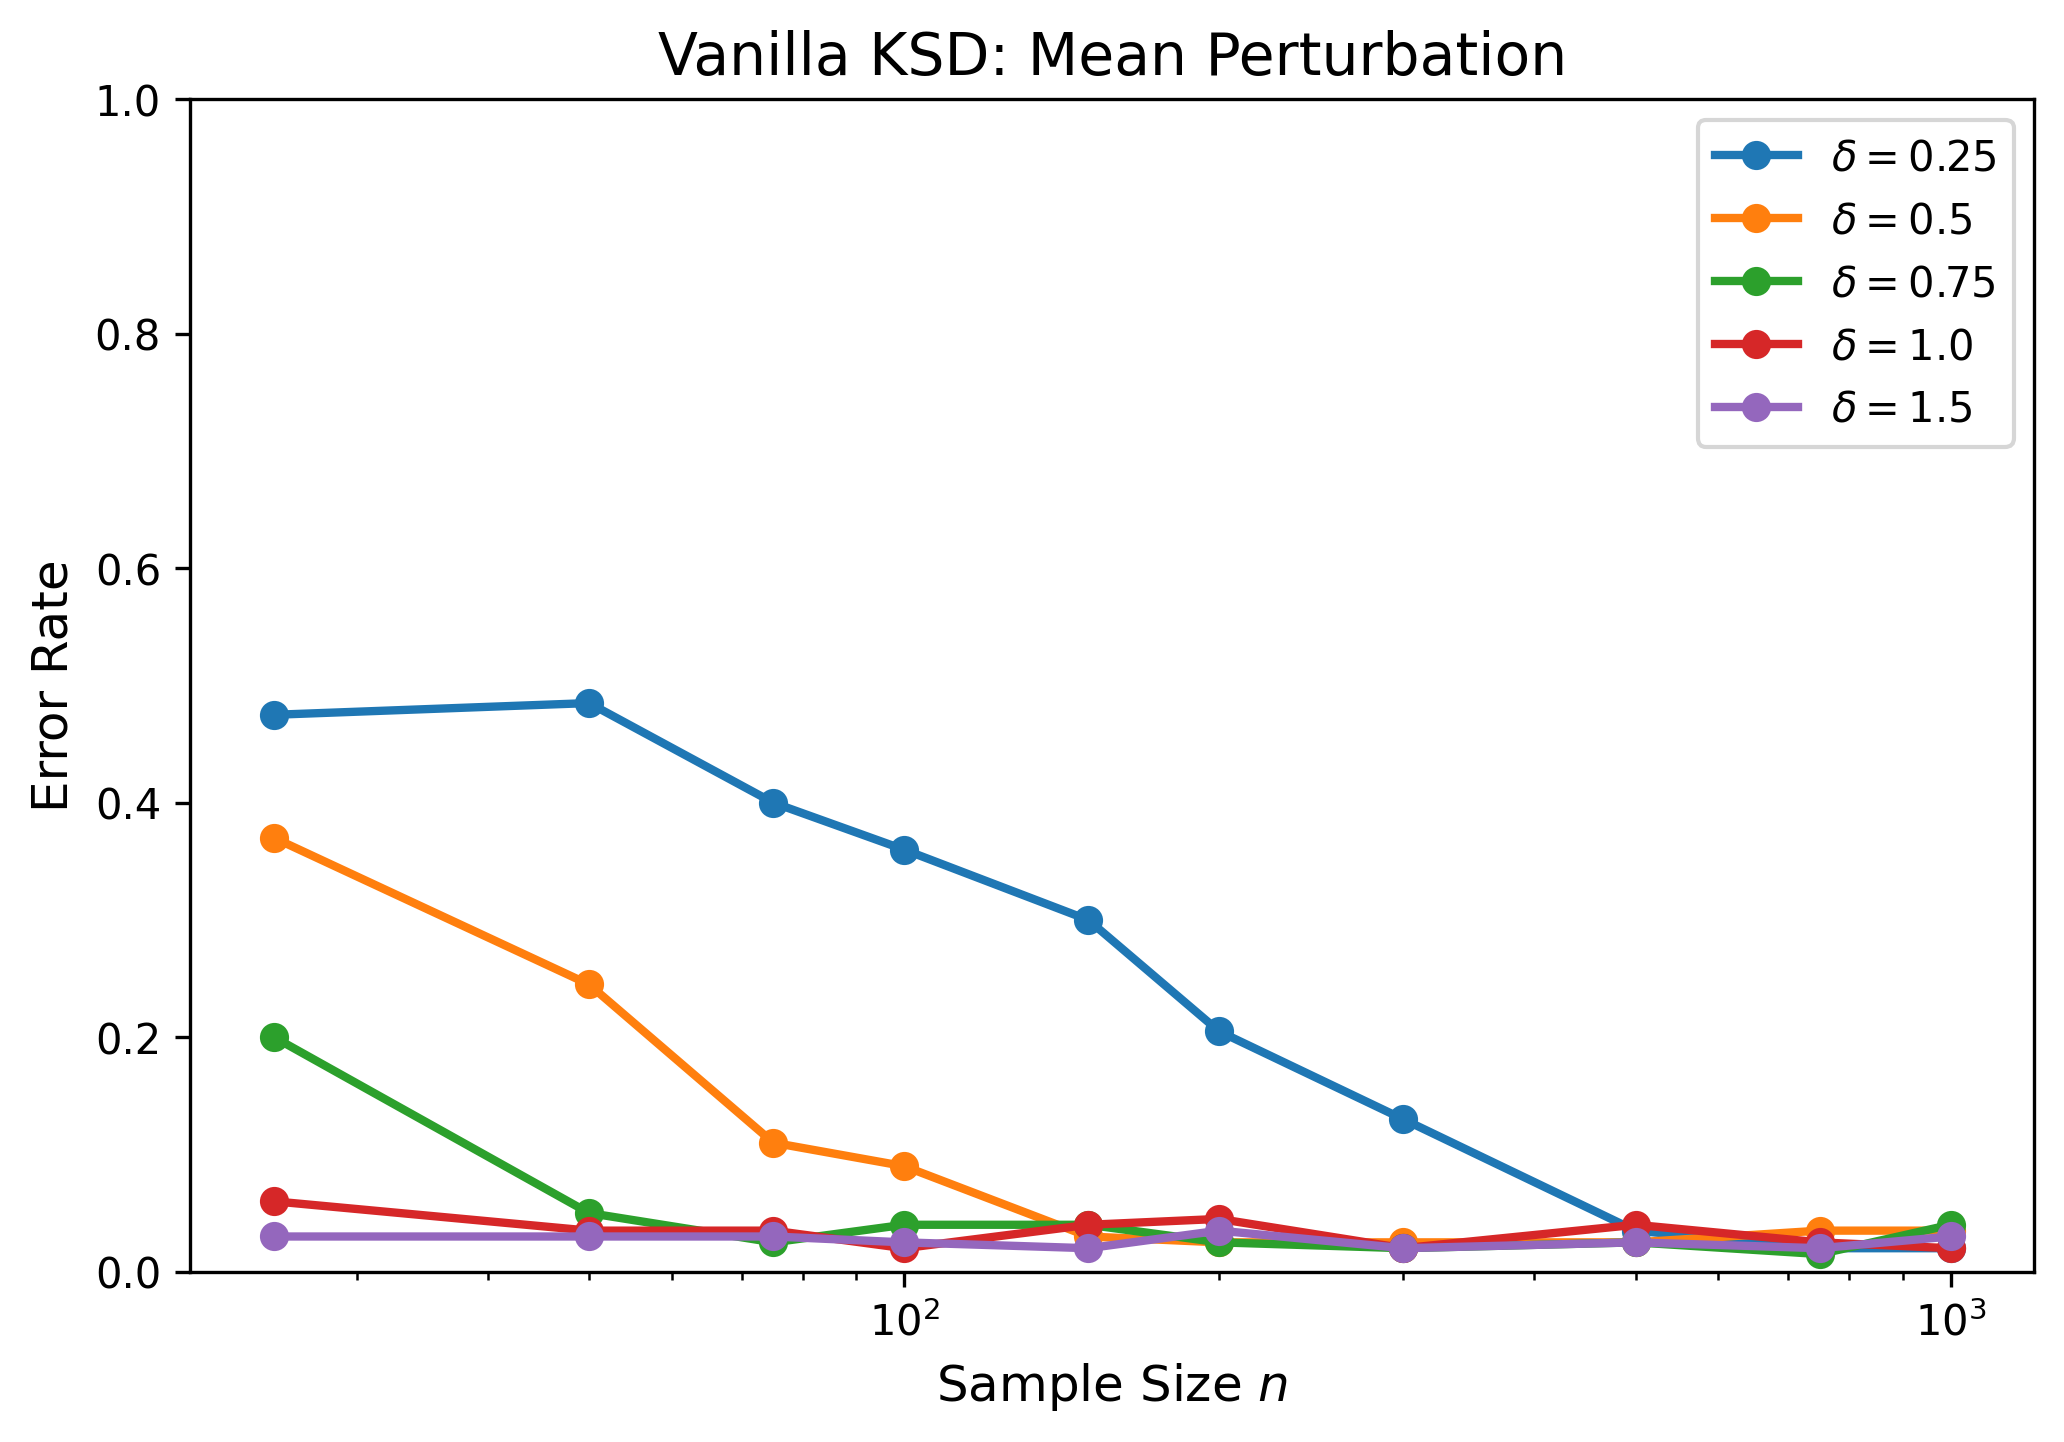
\includegraphics[width=\textwidth]{KSD/Vanilla/vanilla_ksd_mean_perturbation_error_rate.png}
        \caption{}
        \label{fig:roc}
    \end{subfigure}
    \hfill
    \begin{subfigure}{0.45\textwidth}
        \centering
        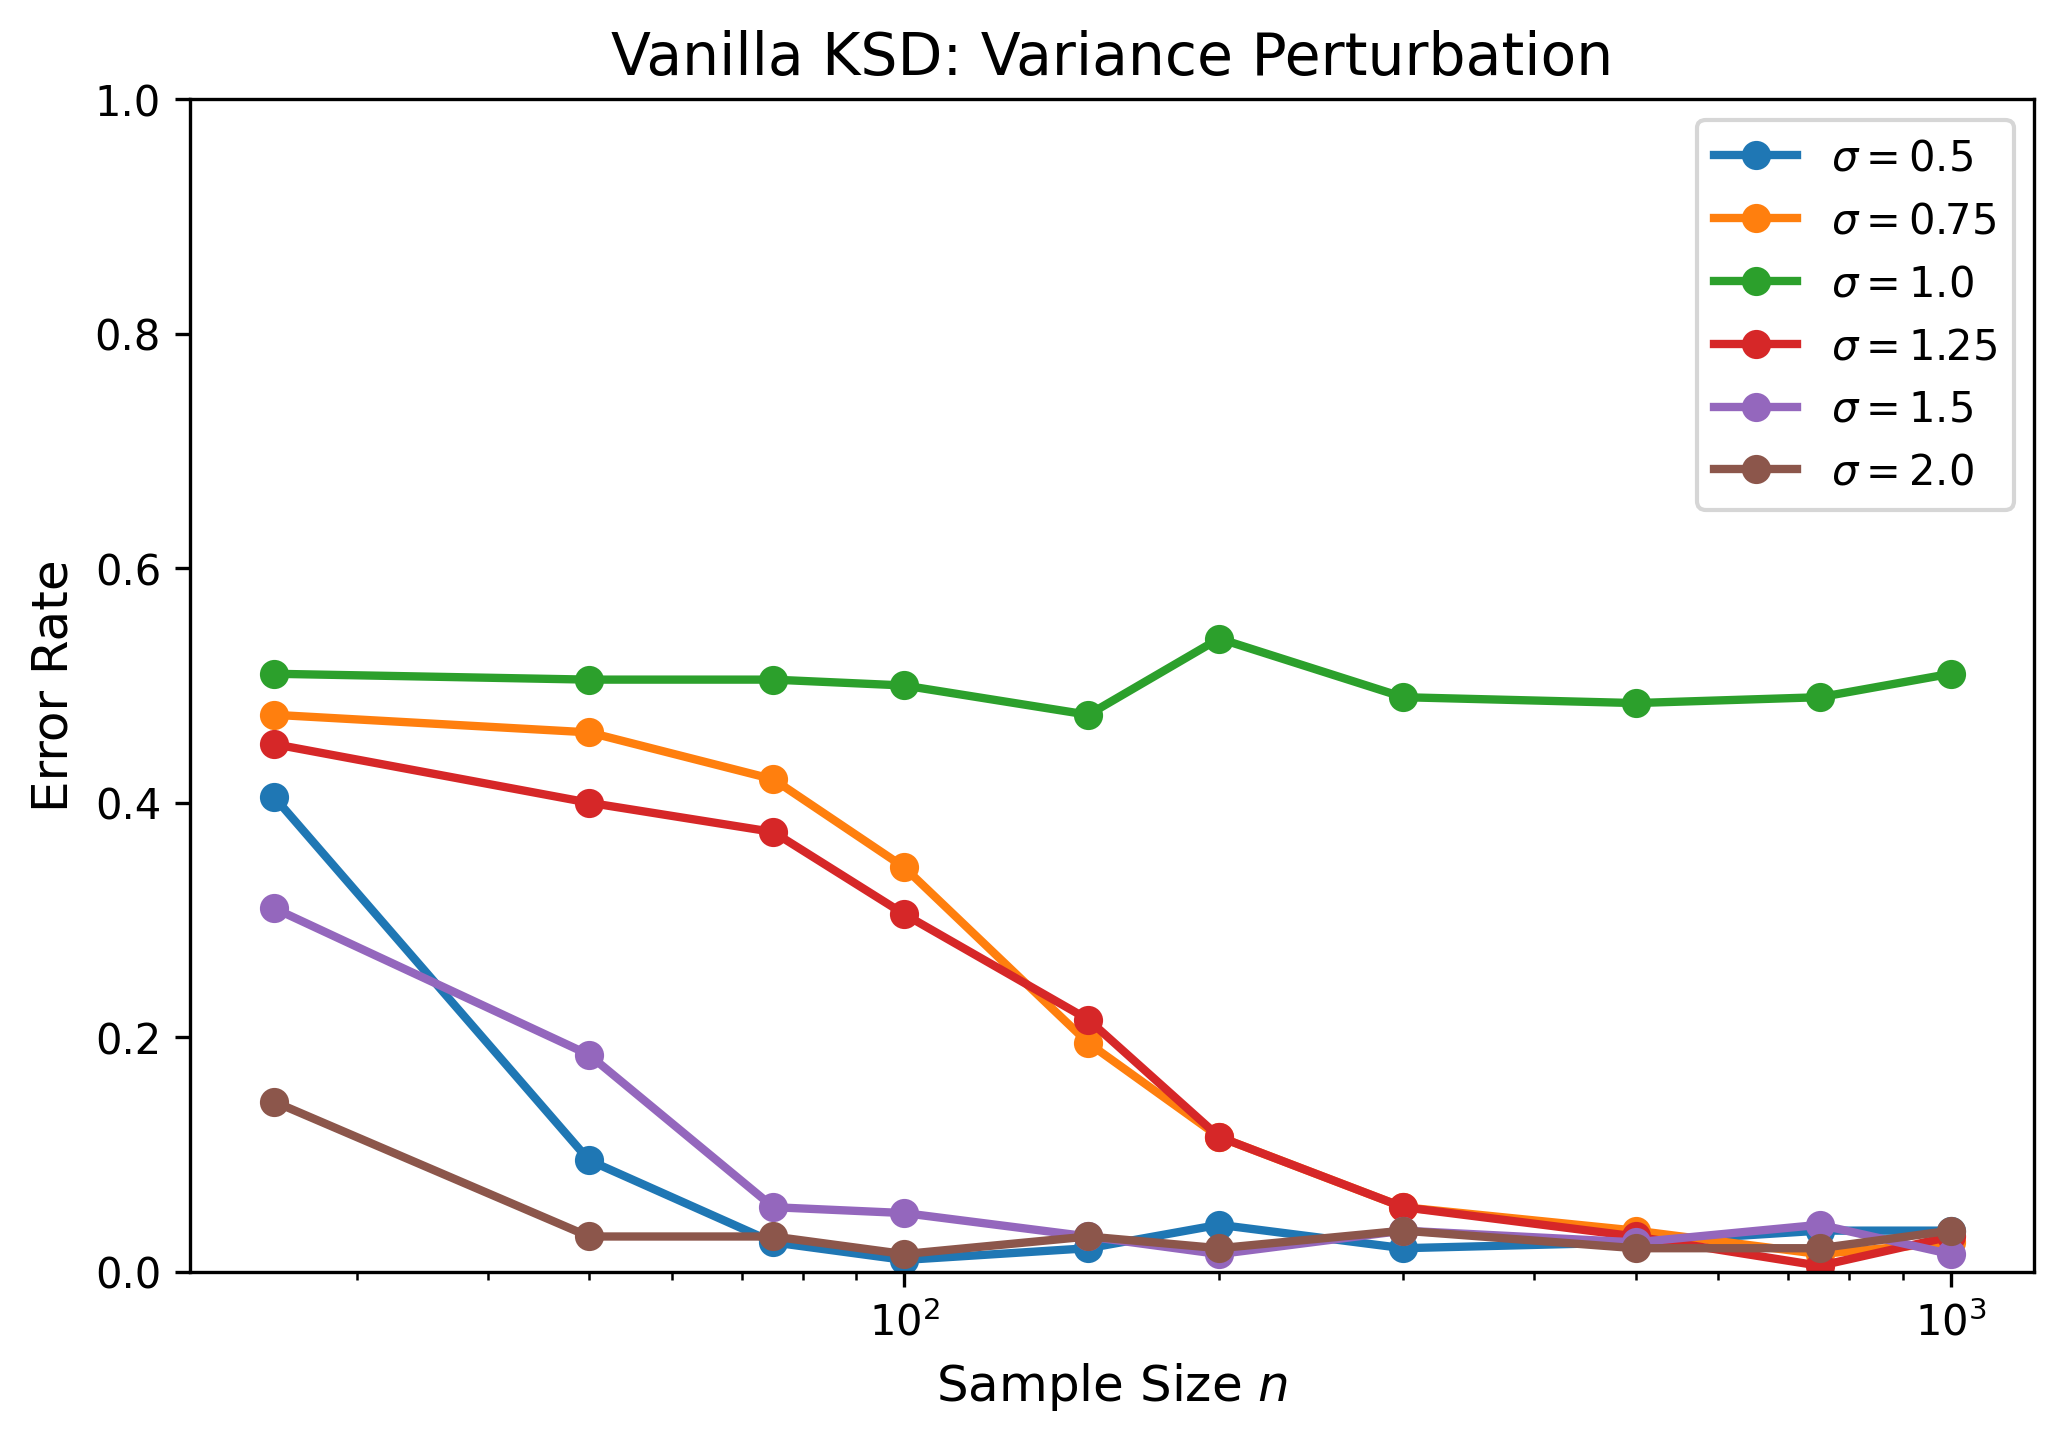
\includegraphics[width=\textwidth]{KSD/Vanilla/vanilla_ksd_variance_perturbation_error_rate.png}
        \caption{}
        \label{fig:power}
    \end{subfigure}

    \vspace{0.5cm}

    % Second row
    \begin{subfigure}{0.45\textwidth}
        \centering
        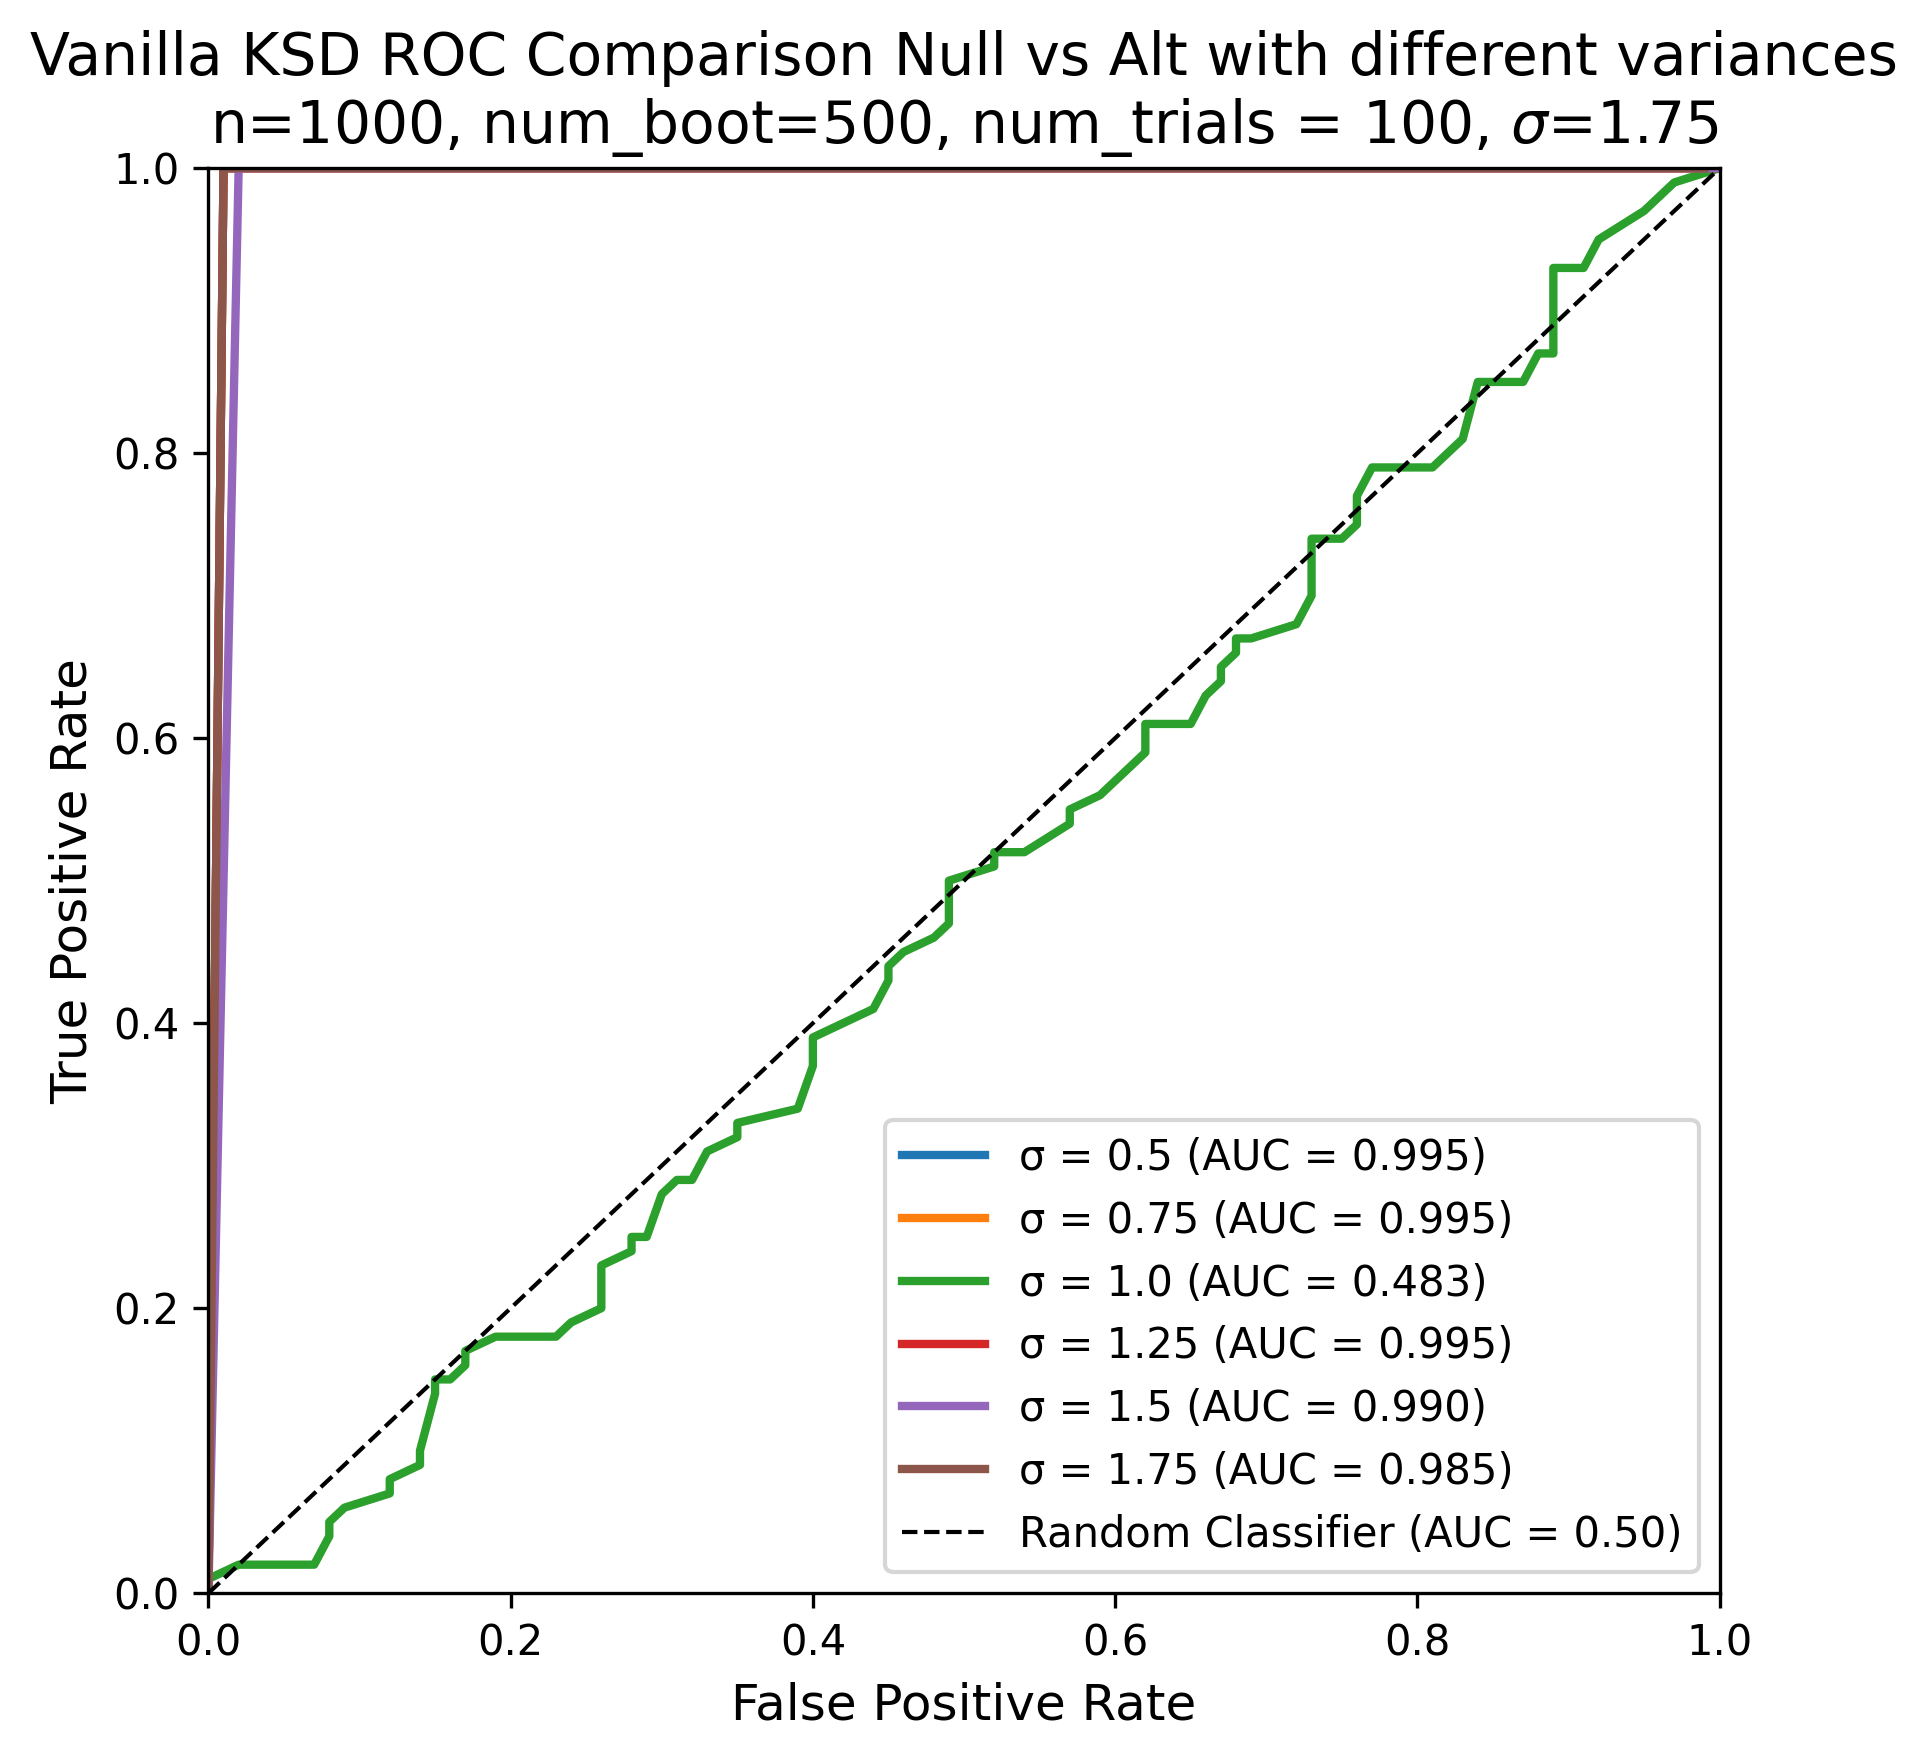
\includegraphics[width=\textwidth]{KSD/Vanilla/vanilla_ksd_roc_comparison_different_sigmas.png}
        \caption{}
        \label{fig:mse}
    \end{subfigure}
    \hfill
    \begin{subfigure}{0.45\textwidth}
        \centering
        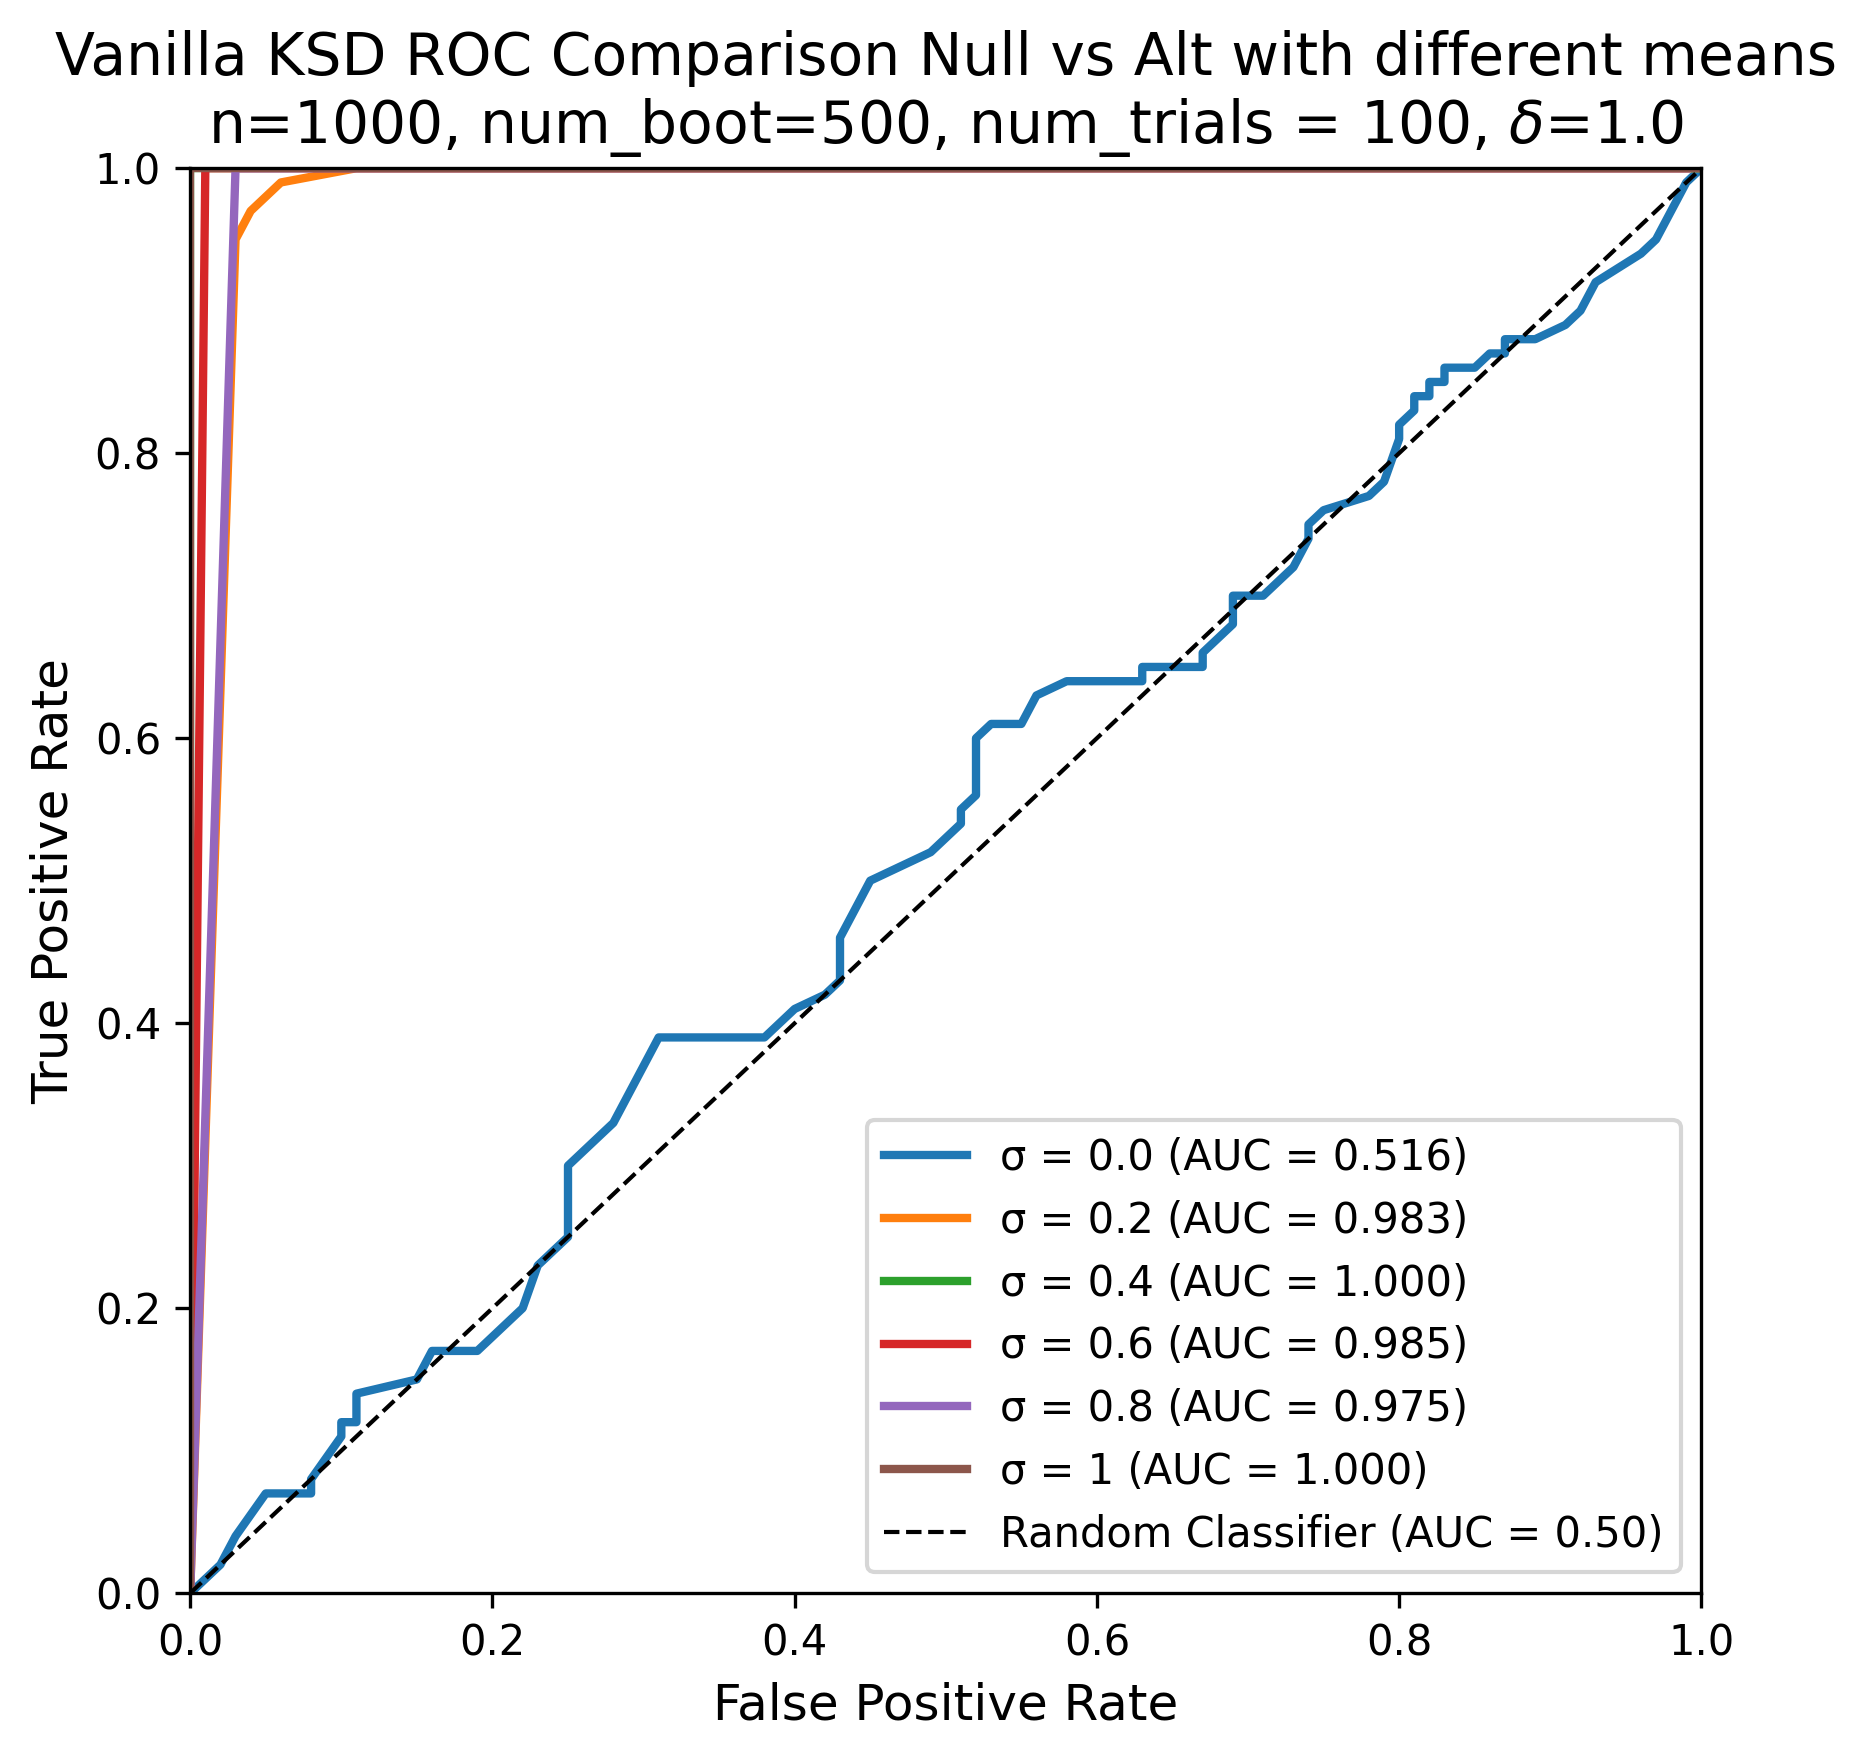
\includegraphics[width=\textwidth]{KSD/Vanilla/vanilla_ksd_roc_comparison_different_deltas.png}
        \caption{}
        \label{fig:variance}
    \end{subfigure}

    \vspace{0.5cm}

    % Third row - centered single image
    \begin{subfigure}{0.45\textwidth}
        \centering
        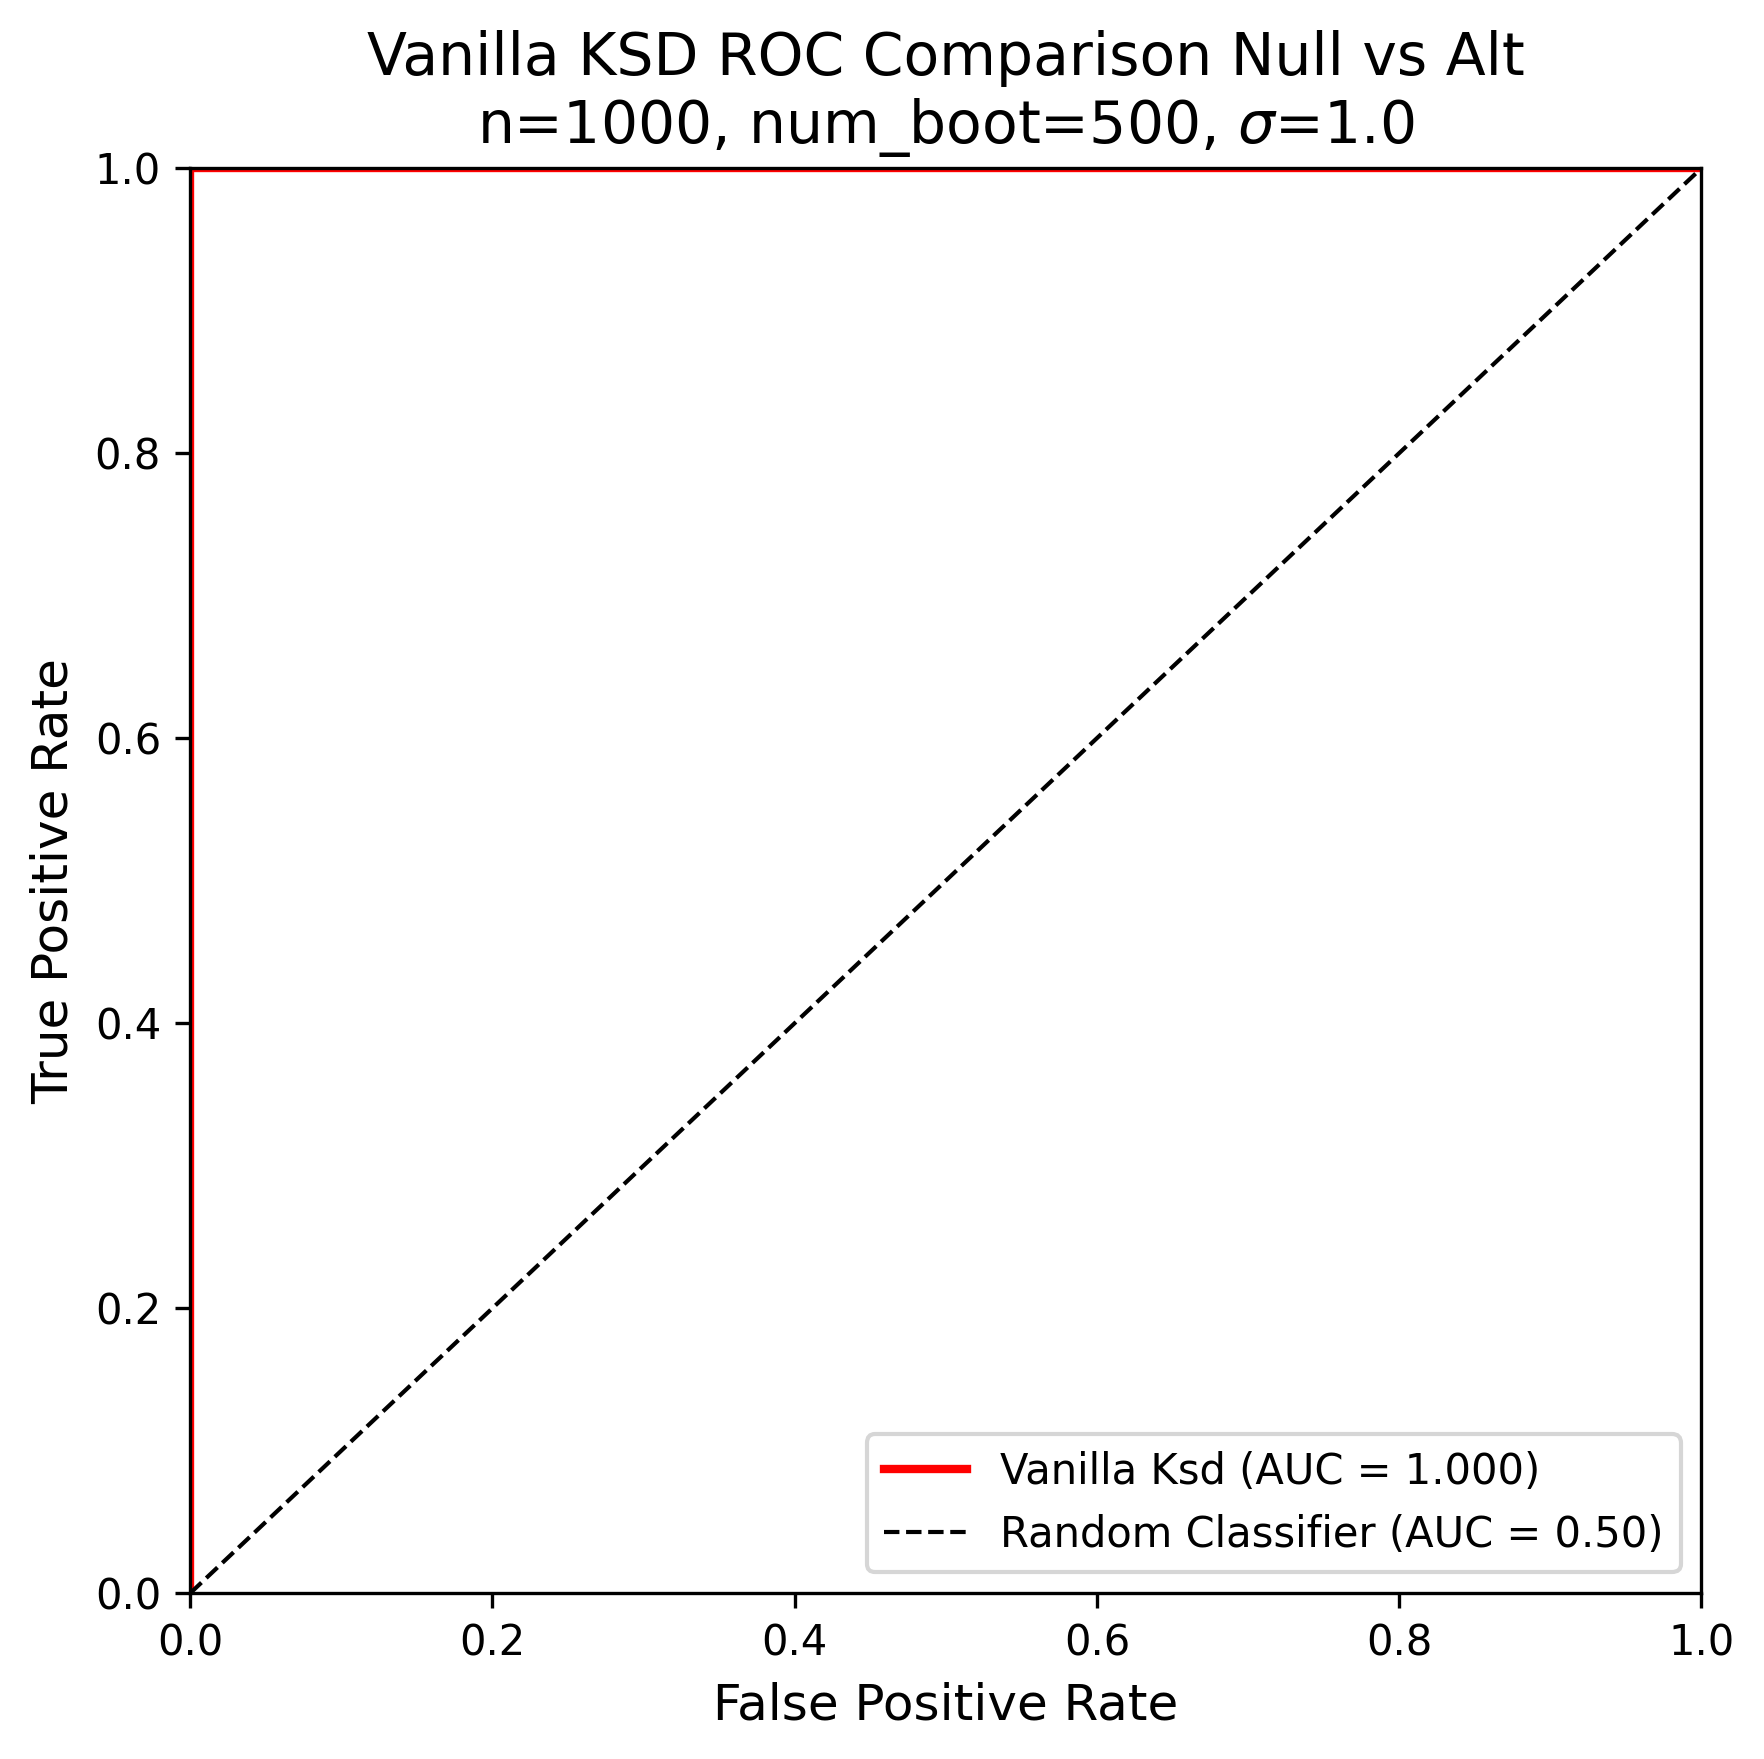
\includegraphics[width=\textwidth]{KSD/Vanilla/vanilla_ksd_roc_comparison.png}
        \caption{}
        \label{fig:bias}
    \end{subfigure}

    \caption{Comparison of the proposed method under different experimental settings.}
    \label{fig:results}
\end{figure}

\chapter{Score Matching technique on KSD Framework}
\section{Score Matching Objective}
For simple distributions which are tractable, we can easily find the score function and use it analytically. It acts as a sanity check for any algorithm. However for distributions that are intractable, finding the score becomes difficult. We use score matching techniques that utilizes a neural network to train the score function to be used later. We use, in our work the score matching techniques using stochastic differential equations \cite{song2021scorebasedgenerativemodelingstochastic}. For training purpose, we use forward SDE .

\begin{equation}
\mathrm{d}x = f(x,t)\,\mathrm{d}t + g(t)\,\mathrm{d}w
\end{equation}.

\noindent
Following the paper \cite{song2021scorebasedgenerativemodelingstochastic} and tutorial based on it, we use
\begin{equation}
   d {x} = \sigma^t d\mathbf{w}, \quad t\in[0,1]
\end{equation}

\noindent
to follow the SDE. We then draw samples from $x(t) \sim q_(x)$ and perturb it with $x_t = x_0 + \sigma_t z$, $z \sim \mathcal{N}(0,I)$. We then choose $\sigma^t$ as follows
\begin{equation}
    \sigma_t =
    \left(
        \frac{\sigma^{2t} - 1}{2\log \sigma}
    \right)^{1/2}
\end{equation}

\noindent
The perturbed distribution becomes
\begin{equation}
    q_{0t}({x}(t) \mid {x}(0)) = \mathcal{N}\bigg({x}(t); {x}(0), \frac{1}{2\log \sigma}(\sigma^{2t} - 1) \mathbf{I}\bigg)
\end{equation}

\noindent
We can approximate the score function as
\begin{equation}
s_{\theta}(x_t,t) \approx \nabla_{x_t}\log q_t(x_t).
\label{eq:score_approx}
\end{equation}

\noindent
However we only have the access to the perturbed  conditioned true samples. Using marginals and expectation, we can approximate the marginals i.e. our perturbed samples as conditional score. The conditional score is
\begin{align}
\nabla_{x_t}\log q_{0t}(x_t\mid x_0)
&=
-\frac{1}{2\sigma_t^2}
\nabla_{x_t}\|x_t-x_0\|^2 \\
&=
-\frac{1}{\sigma_t^2}(x_t-x_0)\\
&=
-\frac{z}{\sigma_t}.
\label{eq:denoise_score}
\end{align}

\noindent
We then make use of Eq. ($7$) \cite{song2021scorebasedgenerativemodelingstochastic} for training our score function, given as 
\begin{equation}
\theta^*
=
\underset{\theta}{\arg\min}\;
\mathbb{E}_t
\left\{
\sigma_t
\mathbb{E}_{x_0}
\mathbb{E}_{x_t\mid x_0}
\left[
\left\|
s_{\theta}(x(t),t)
-
\nabla_{x(t)}
\log q_{0t}(x_t\mid x_t)
\right\|_2^2
\right]
\right\}.
\label{eq:score_training}
\end{equation}

\noindent
We then use \ref{eq:denoise_score} in \ref{eq:score_training} for our training of the model. After we get this trained score model we plug the trained score in \ref{eq:u_q} which becomes
\begin{equation}
\begin{aligned}
u_{\theta}(x,x';t)
={}& s_{\theta}(x,t)^\top k(x,x')s_{\theta}(x',t) \\
&+ s_{\theta}(x,t)^\top \nabla_{x'} k(x,x') \\
&+ \nabla_x k(x,x')^\top s_{\theta}(x',t) \\
&+ \operatorname{tr}\left(\nabla_{x,x'} k(x,x')\right).
\end{aligned}
\end{equation}

\section{Experiment}
We now use the training objective on the MNIST dataset. We train the score on the MNIST even training dataset and now we use the score based KSD framework on the following hypothesis: Null - even digits vs Alternate - odd digits. The selection of $\sigma$ and timestep $t$ are our hyper-parameters. We follow \cite{song2021scorebasedgenerativemodelingstochastic} and keep $\sigma = 25$. However to get the best possible results, we take $t \in (0.00001, 1)$ logarithmically. We then focus near the region $t=0.1$ and then do further experiments to narrow it down to $t \in \{0.25,\,0.27,\,0.3,\,0.33,\,0.35,\,0.37,\,0.4\}$. 200 bootstrap samples along with 128 original samples across 100 trials are taken in account. The AUC Results are given below.
\begin{table}[ht]
    \centering
    \caption{AUC values for different values of $t$.}
    \label{tab:auc_t}
    \begin{tabular}{cc}
        \hline
        Timestep $t$ & AUC \\
        \hline
        0.25 & 0.862 \\
        0.27 & 0.865 \\
        0.30 & 0.942 \\
        0.33 & 0.939 \\
        0.35 & 0.920 \\
        0.37 & 0.947 \\
        0.40 & 0.947 \\
        \hline
    \end{tabular}
\end{table}

\noindent
We then perform the power test on null and alternate samples to test the statistical power of the tests. The results are provided in the Fig \ref{fig_ROC_power_MNIST}

\begin{figure}[htbp]
    \centering
    % First row
    \begin{subfigure}{0.45\textwidth}
        \centering
        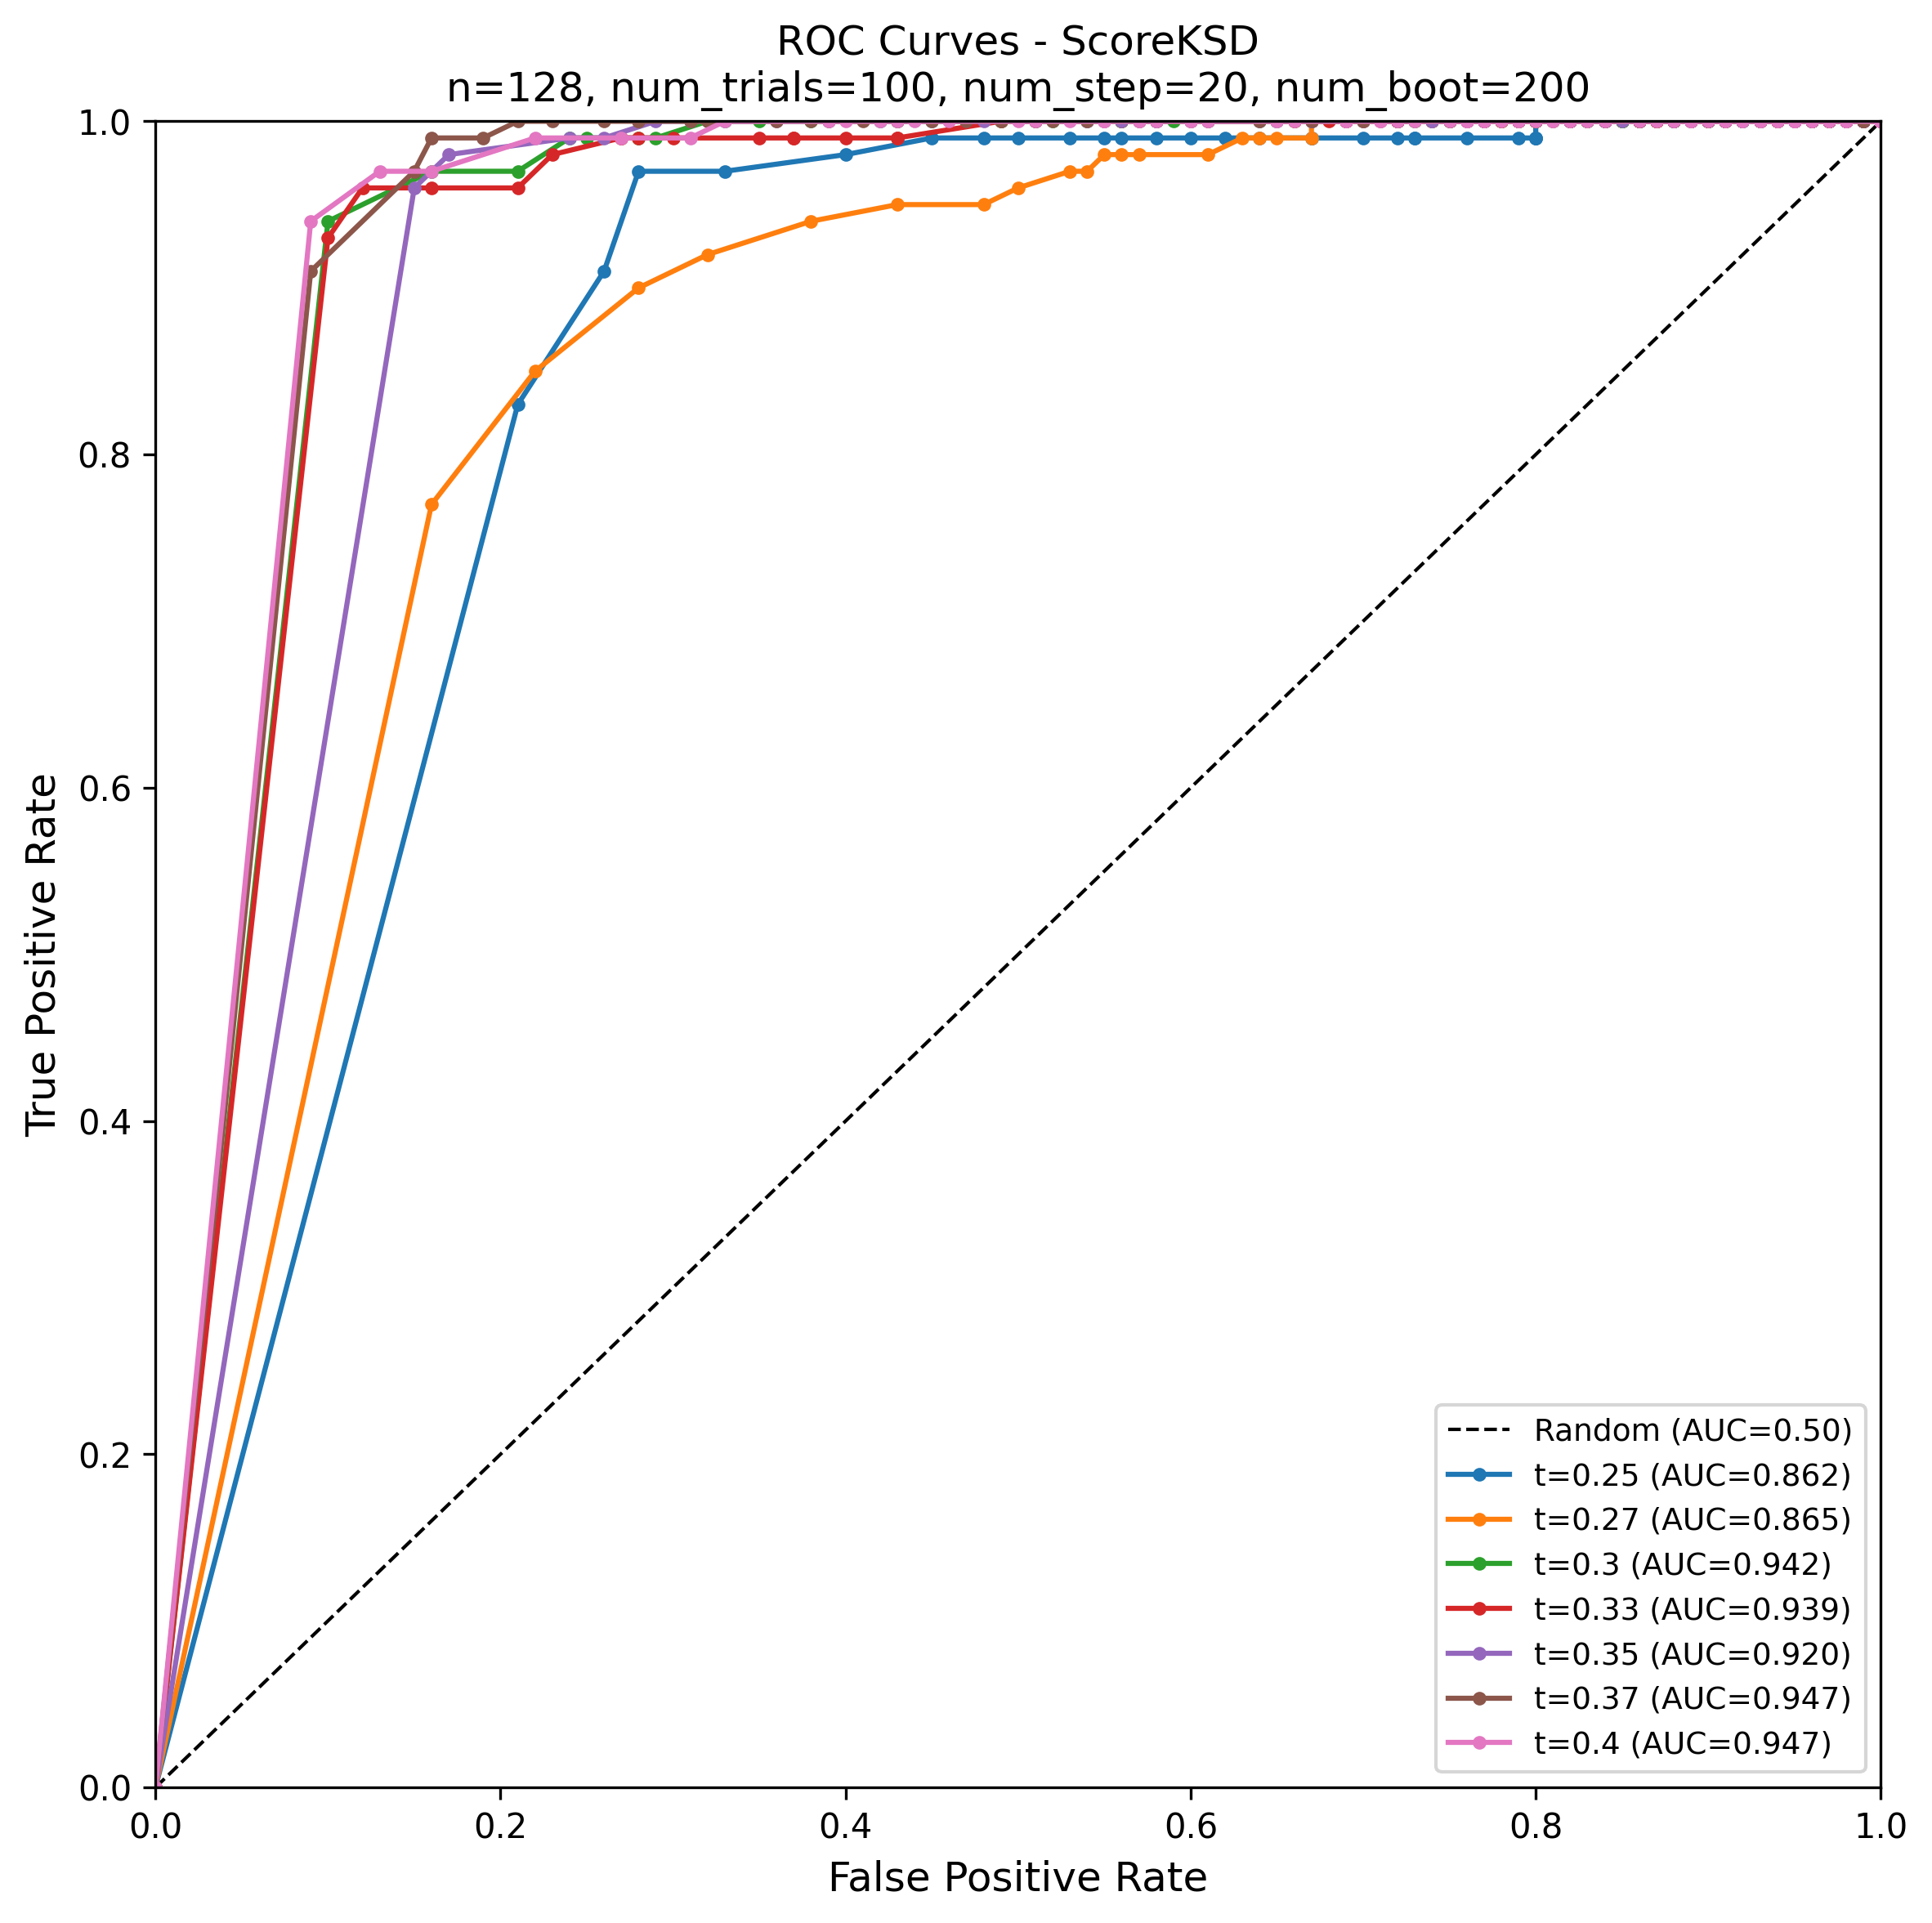
\includegraphics[width=\textwidth]{KSD/MNIST/roc_curve_scoreksd.png}
        \label{fig:mnist_roc}
        \caption{}
    \end{subfigure}
    \hfill
    \begin{subfigure}{0.45\textwidth}
        \centering
        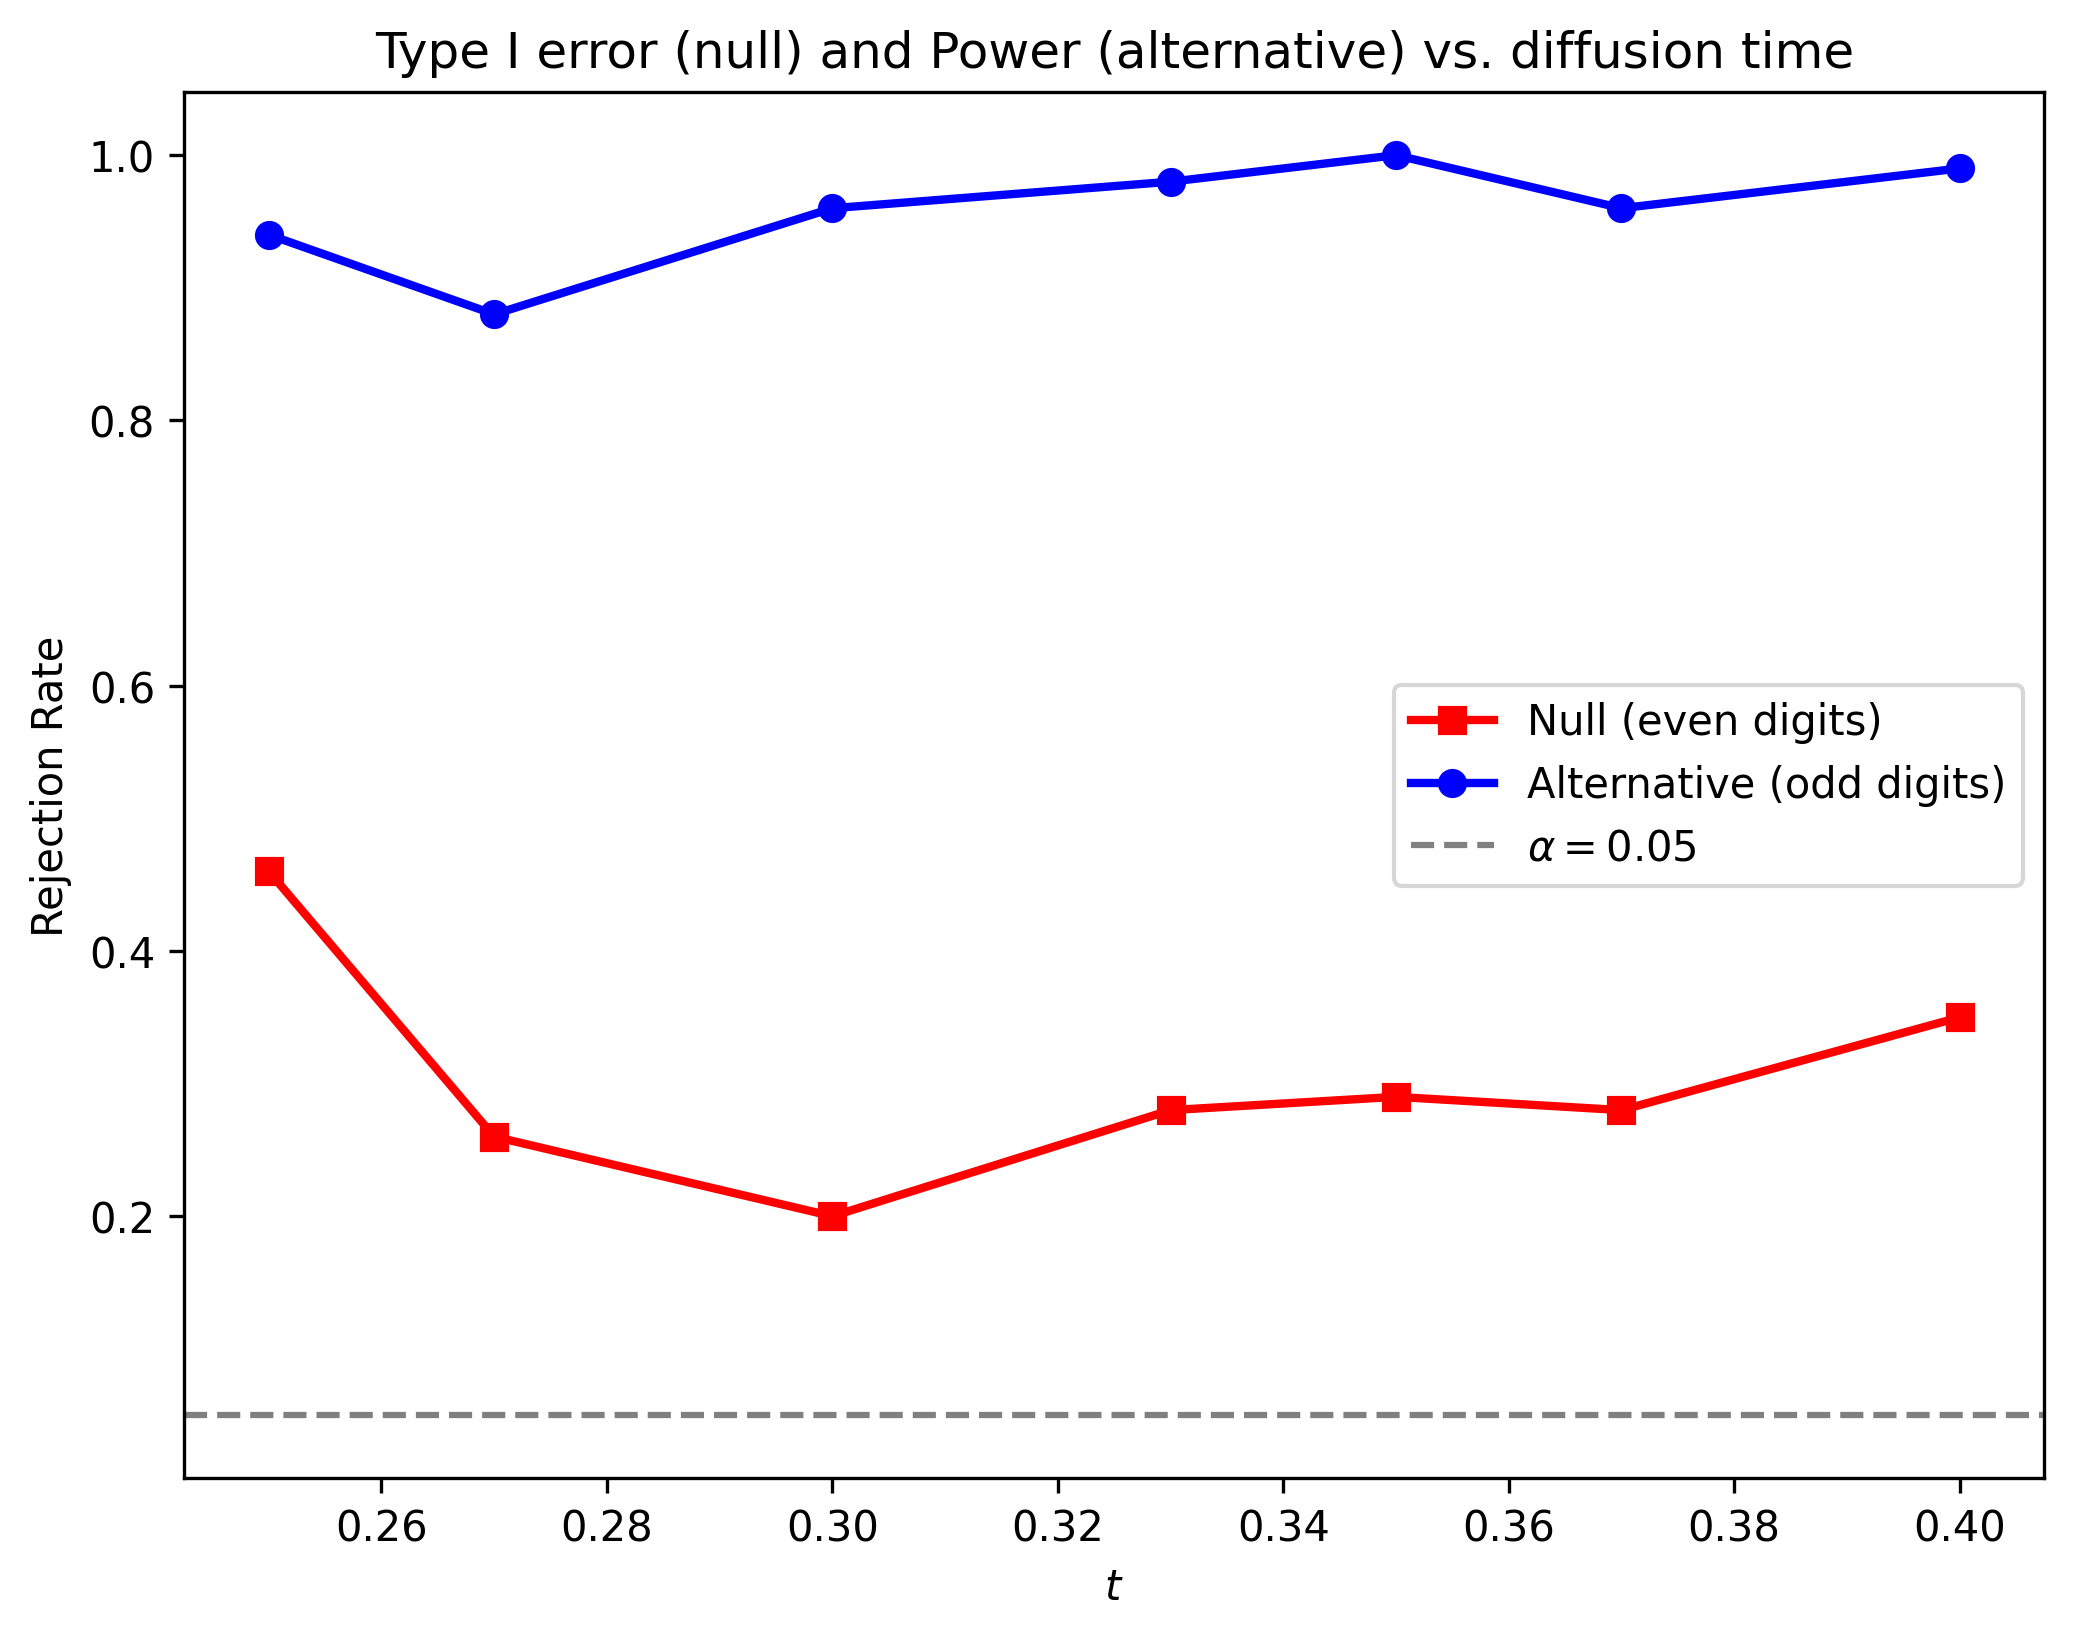
\includegraphics[width=\textwidth]{KSD/MNIST/combined_ksd_null_alt.png}
        \label{fig:mnist_power}
        \caption{}
    \end{subfigure}
    \caption{ROC Curves $(a)$ and the Power plots $(b)$ for MNIST Even vs Odd samples}
    \vspace{0.5cm}
    \label{fig_ROC_power_MNIST}
\end{figure}

\section{Discussion}
The score based KSD framework works well for MNIST dataset. It is also able to reasonably perform well on the power tests for null and alternate. However the power is still not close to the desired level for both.

\vspace{0.3cm}
\noindent
There are two problems that are arising: selection of $\sigma$ and $t$. For other datasets, we might have to tune it, but given the increase in dimension it is still now clear how computationally expensive it might become.

\chapter{Diffusion Posterior Sampling}

\section{Preliminaries}
Now that we have a trained score model, we want to generate samples based on that. We get our inspiration from diffusion posterior sampling, which is used in noisy inverse problems. In such case, we want to get an estimate of the clean images when conditioned on the noisy observation \cite{chung2024diffusionposteriorsamplinggeneral}. The paper uses discrete denoising process, this work tries to implement Euler - Maruyama process, discussed in \cite{song2021scorebasedgenerativemodelingstochastic}
\section{Diffusion Posterior Sampling}
We first consider an inverse problem of the form
\begin{equation}
    y = \mathcal{A}(x_0) + \epsilon,
\end{equation}

\noindent
where $x_0$ denotes the unknown clean image, $\mathcal{A}$ is a measurement operator, $y$ is the observed measurement, and $\epsilon$ represents measurement noise. Our  objective is to generate samples from the posterior distribution
\begin{equation}
    q(x_0 \mid y)
    \propto
    q(y \mid x_0)p(x_0).
\end{equation}

\noindent
A score-based model provides an estimate of the score of the perturbed data distribution which we have already done,
\begin{equation}
    s_\theta(x_t,t)
    \approx
    \nabla_{x_t}\log q_t(x_t),
\end{equation}

\noindent
where $p_t(x_t)$ denotes the marginal distribution of the data at diffusion time $t$ \ref{eq:score_approx}.

\subsection{Forward Perturbation Process and Training}
This process has been used in training the score network (See Section 3.1). 

\subsection{Reverse-Time Sampling}
Once the score network has been trained, samples can be generated by solving the reverse-time SDE. The reverse-time SDE is
\begin{equation}
    dx
    =
    \left[
    f(x,t)-g(t)^2
    \nabla_x\log p_t(x)
    \right]dt
    +
    g(t)d\overline{W}_t,
\end{equation}

\noindent
where time is integrated from $T$ towards $0$ \cite{song2021scorebasedgenerativemodelingstochastic}.

\vspace{0.3cm}
\noindent
Replacing the unknown score by the trained score network gives
\begin{equation}
    dx
    =
    \left[
    f(x,t)-g(t)^2s_\theta(x,t)
    \right]dt
    +
    g(t)d\overline{W}_t.
\end{equation}

\noindent
In the implementation, an Euler-Maruyama discretization is used. With a reverse time step $\Delta t>0$, the update is
\begin{equation}
    x_{t-\Delta t}'
    =
    x_t
    +
    g(t)^2s_\theta(x_t,t)\Delta t
    +
    g(t)\sqrt{\Delta t}\,z,
\end{equation}
where $z\sim\mathcal{N}(0,I).$

\subsection{Tweedie's Estimate}
At each diffusion time, an estimate of the corresponding clean image is obtained using Tweedie's formula:
\begin{equation}
    \hat{x}_0
    =
    x_t+\sigma_t^2s_\theta(x_t,t).
\end{equation}

\noindent
This estimate is subsequently used to evaluate the measurement consistency.

\subsection{DPS Correction and step size}
For the inverse problem, the estimated clean image should satisfy
\begin{equation}
    y\approx\mathcal{A}(\hat{x}_0).
\end{equation}

\noindent
A measurement loss is therefore defined as
\begin{equation}
    \mathcal{L}_{\mathrm{meas}}
    =
    \left\|
    y-\mathcal{A}(\hat{x}_0)
    \right\|_2^2.
\end{equation}

\noindent
Since $\hat{x}_0$ depends on $x_t$, the gradient of the measurement loss with respect to the current noisy state is given as
\begin{equation}
    g_{\mathrm{meas}}
    =
    \nabla_{x_t}
    \left\|
    y-\mathcal{A}(\hat{x}_0)
    \right\|_2^2.
\end{equation}

\noindent
The DPS correction moves the reverse-SDE sample in the direction that tries to reduce the measurement error:
\begin{equation}
    x_{t-\Delta t}
    =
    x_{t-\Delta t}'
    -
    \zeta_t
    \nabla_{x_t}
    \left\|
    y-\mathcal{A}(\hat{x}_0)
    \right\|_2^2.
\end{equation}

\noindent
In the paper implementation \cite{chung2024diffusionposteriorsamplinggeneral}, the adaptive guidance step size is
\begin{equation}
    \zeta_t
    =
    \frac{\zeta'}
    {
    \left\|
    y-\mathcal{A}(\hat{x}_0)
    \right\|_2+\epsilon
    },
\end{equation}
\noindent
where $\zeta'$ is a guidance parameter which is defined by us and $\epsilon$ is a small numerical constant.

\section{DPS Algorithm}
\begin{algorithm}[H]
\caption{DPS-Gaussian VE-SDE}
\label{alg:measurement_guided_sampling}
\textbf{Input:} \textbf{y}
\begin{algorithmic}[1]

\STATE Sample $x_1 \sim p_1(x)$, $\zeta'$

\FOR{$t: 1 \rightarrow 0$}
    \STATE $s_t \gets s_{\theta}(x_t,t)$
    \STATE $\hat{x}_0 \gets x_t + \sigma_t^2 s_t$
    \STATE
    $\mathcal{L}_{\mathrm{meas}}
    \gets
    \left\|
    y-\mathcal{A}(\hat{x}_0)
    \right\|^2$
    \STATE
    $g_t
    \gets
    \nabla_{x_t}\mathcal{L}_{\mathrm{meas}}$
    \STATE
    $x'_{t-dt}
    \gets
    x_t + g_t^2 s_t\,dt
    + g_t\sqrt{dt}\,z$
   \STATE
    $\displaystyle
    \zeta_t
    \gets
    \frac{\zeta'}
    {\left\|y-\mathcal{A}(\hat{x}_0)\right\|+\epsilon}$
    \STATE
    $x_{t-dt}
    \gets
    x'_{t-dt}-\zeta_t g_t$
\ENDFOR

\end{algorithmic}
\end{algorithm}

\section{Experiments}
We consider two cases for noising a clean image - Gaussian and Inpainting.

\vspace{0.3cm}
\noindent
In Gaussian setting, we use $\zeta' \in \{0.001, \, 0.005, \,0.01, \,0.05, \,0.1, \,0.5, \,1,\, 5, \,10\}$ and generate diffusion posterior samples. We then compare the clean image with measurement and posterior mean for $\zeta' = 0.5$. We then find PSNR and SSIM values for these different $\zeta'$.

\vspace{0.3cm}
\noindent
In Inpainting setting, we in-paint $20\%$ and we again use the same $\zeta'$ and generate diffusion posterior samples. We then compare the clean image with measurement and posterior mean for $\zeta' = 0.1$. We then find PSNR and SSIM values for these different $\zeta'$.

\subsection{Gaussian}
\begin{figure}[H]
    \centering
    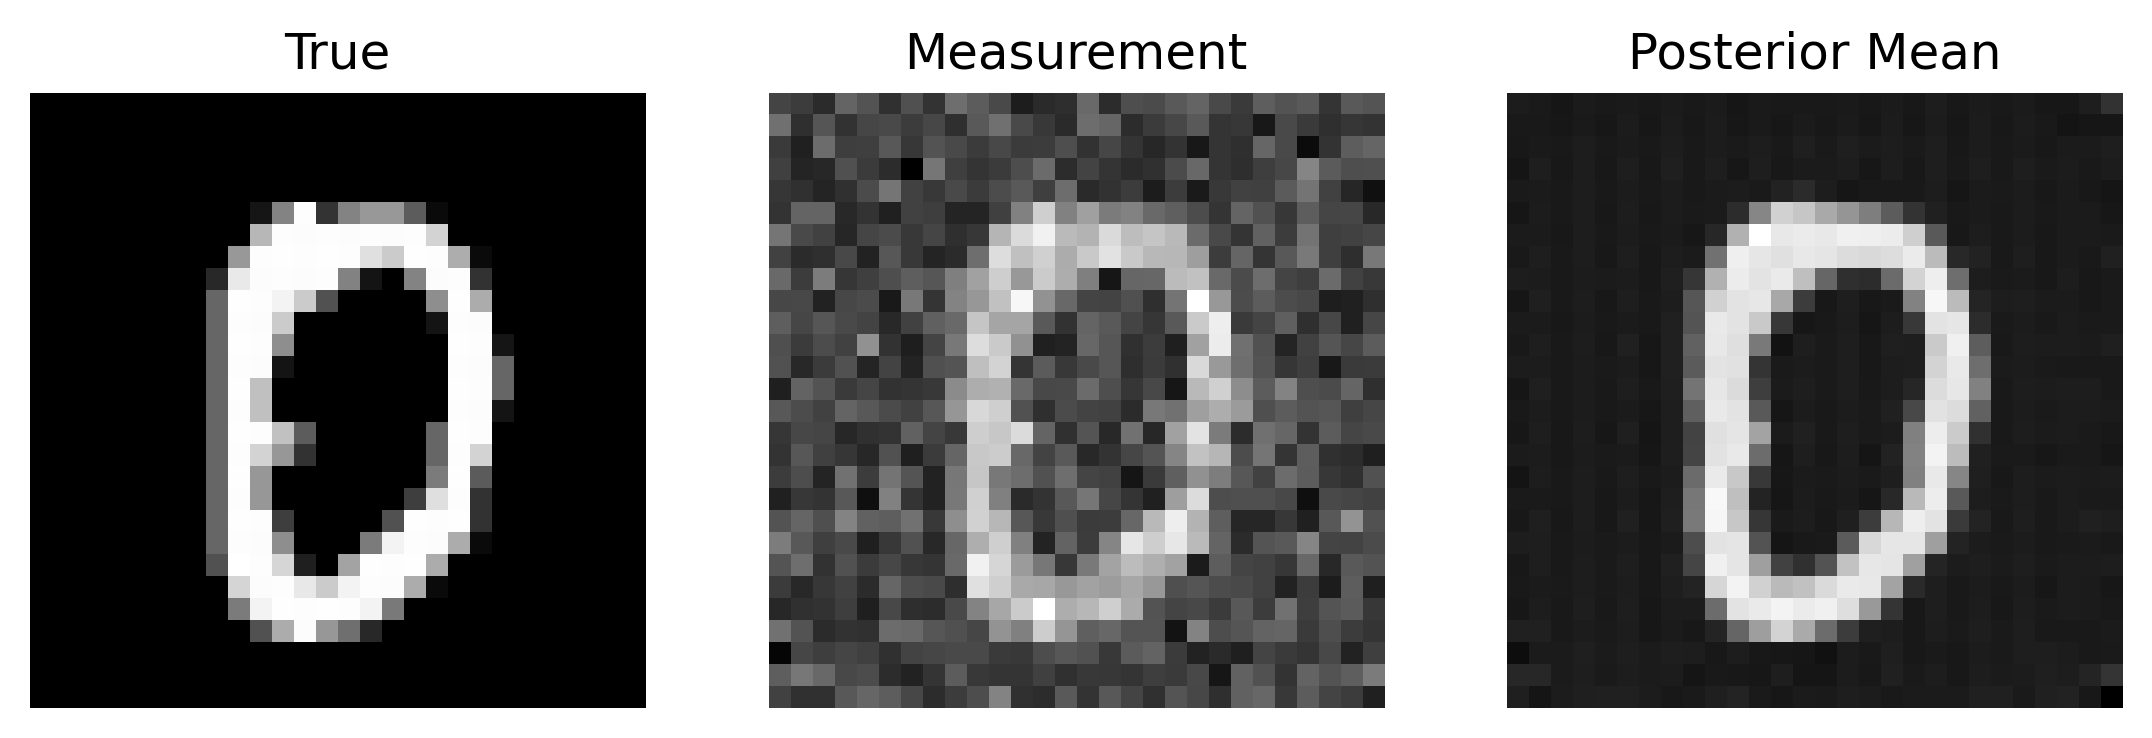
\includegraphics[width=0.8\textwidth]{DPS_VESDE/MNIST/Gauss/Gaussian_posterior_mean_single_digit.png}
    \caption{Clean, Measurement and Posterior Mean}
    \label{fig:gauss_single_mnist}
\end{figure}

\begin{figure}[H]
    \centering
    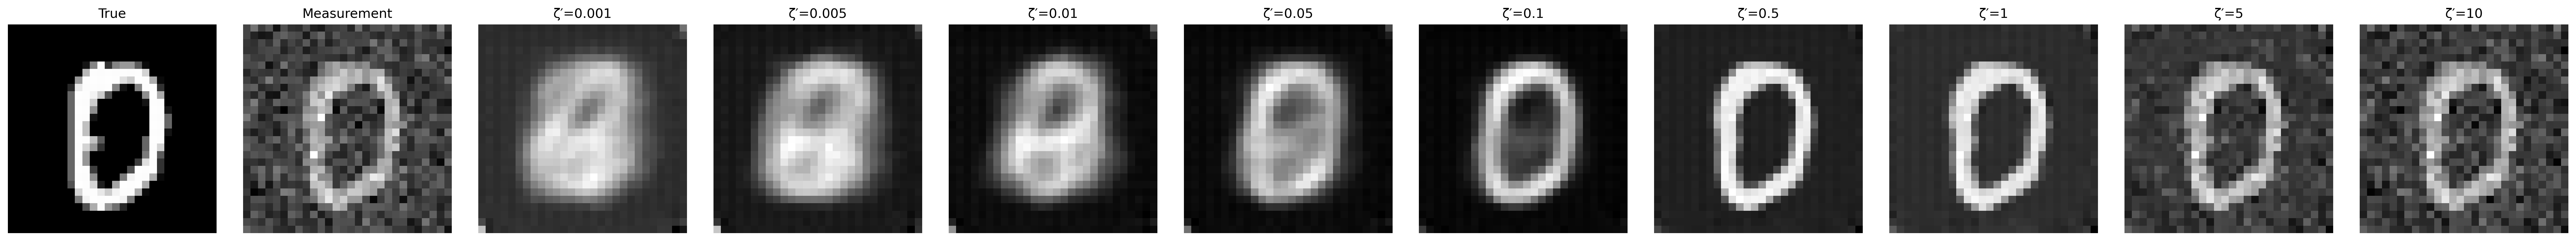
\includegraphics[width=1.0\textwidth]{DPS_VESDE/MNIST/Gauss/Gaussian_posterior_mean_different_zeta_prime.png}
    \caption{Posterior mean images for different $\zeta'$}
    \label{fig:gauss_mnist_zeta_diff}
\end{figure}

\begin{figure}[htbp]
    \centering
    % First row
    \begin{subfigure}{0.45\textwidth}
        \centering
        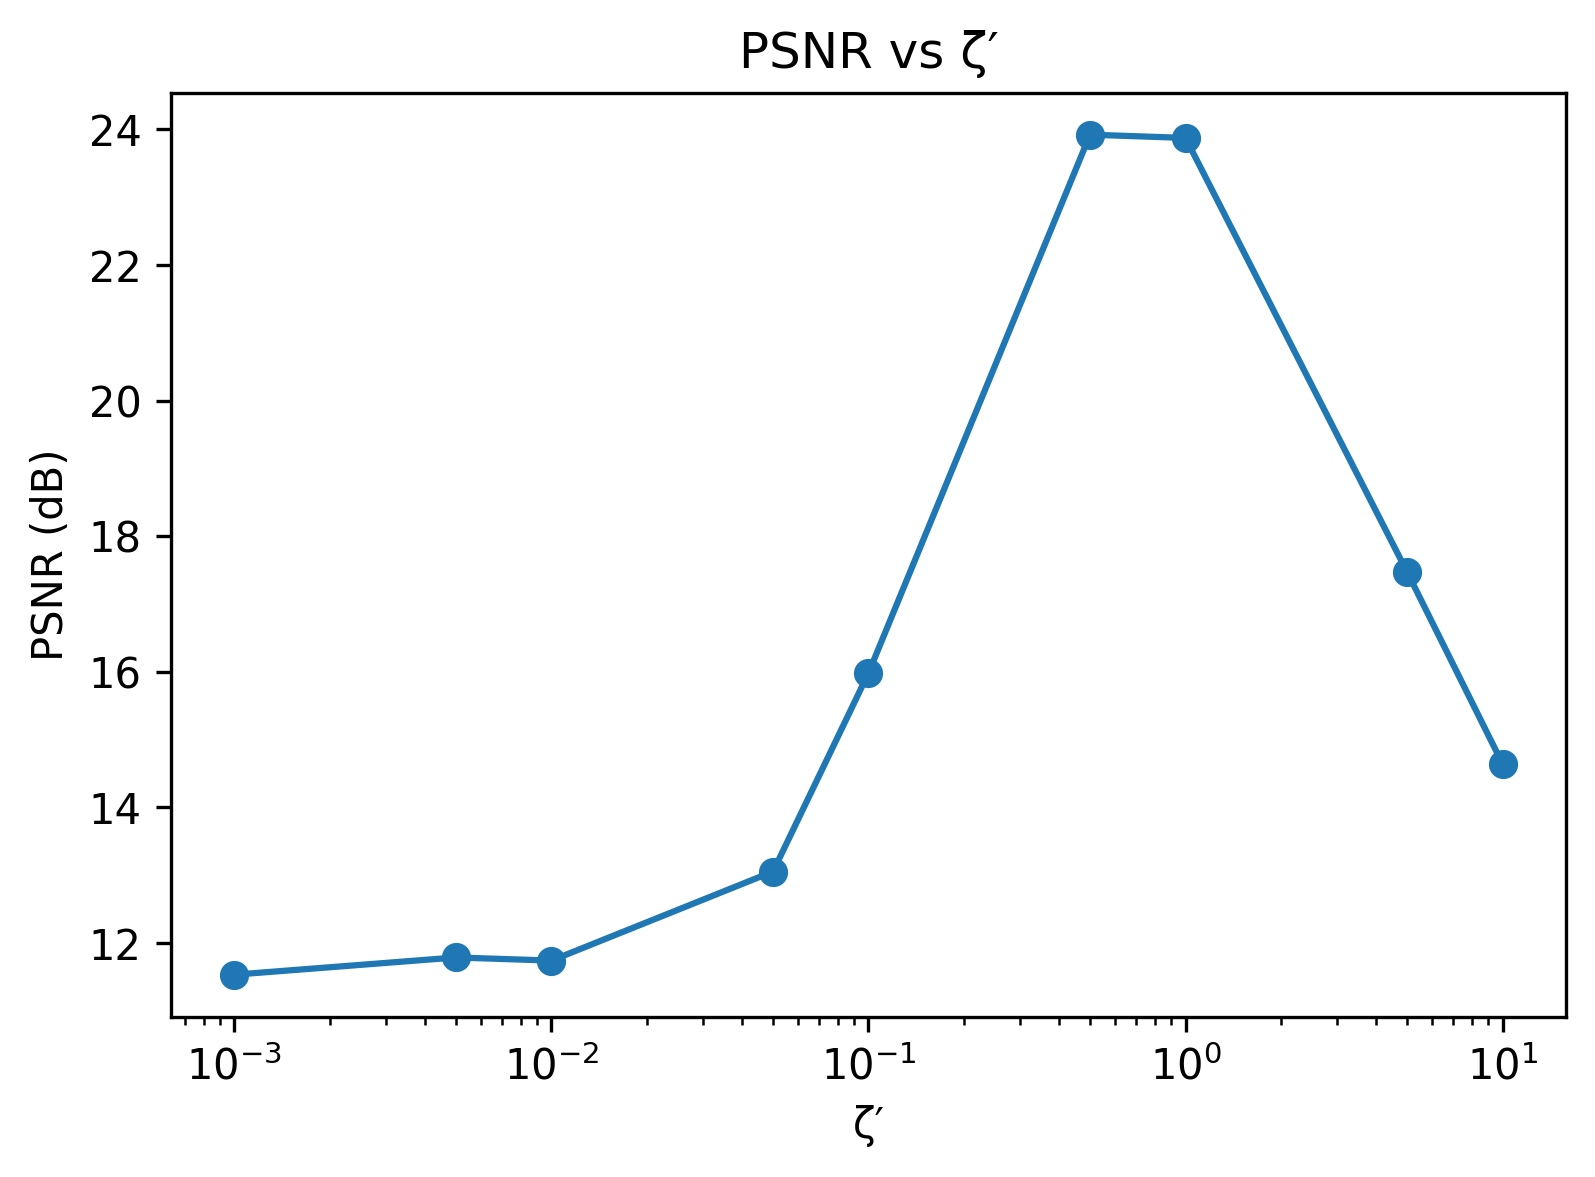
\includegraphics[width=\textwidth]{DPS_VESDE/MNIST/Gauss/PSNR_Gaussian_dps.png}
        \caption{Gaussian PSNR}
        \label{fig:psnr_gauss}
    \end{subfigure}
    \hfill
    \begin{subfigure}{0.45\textwidth}
        \centering
        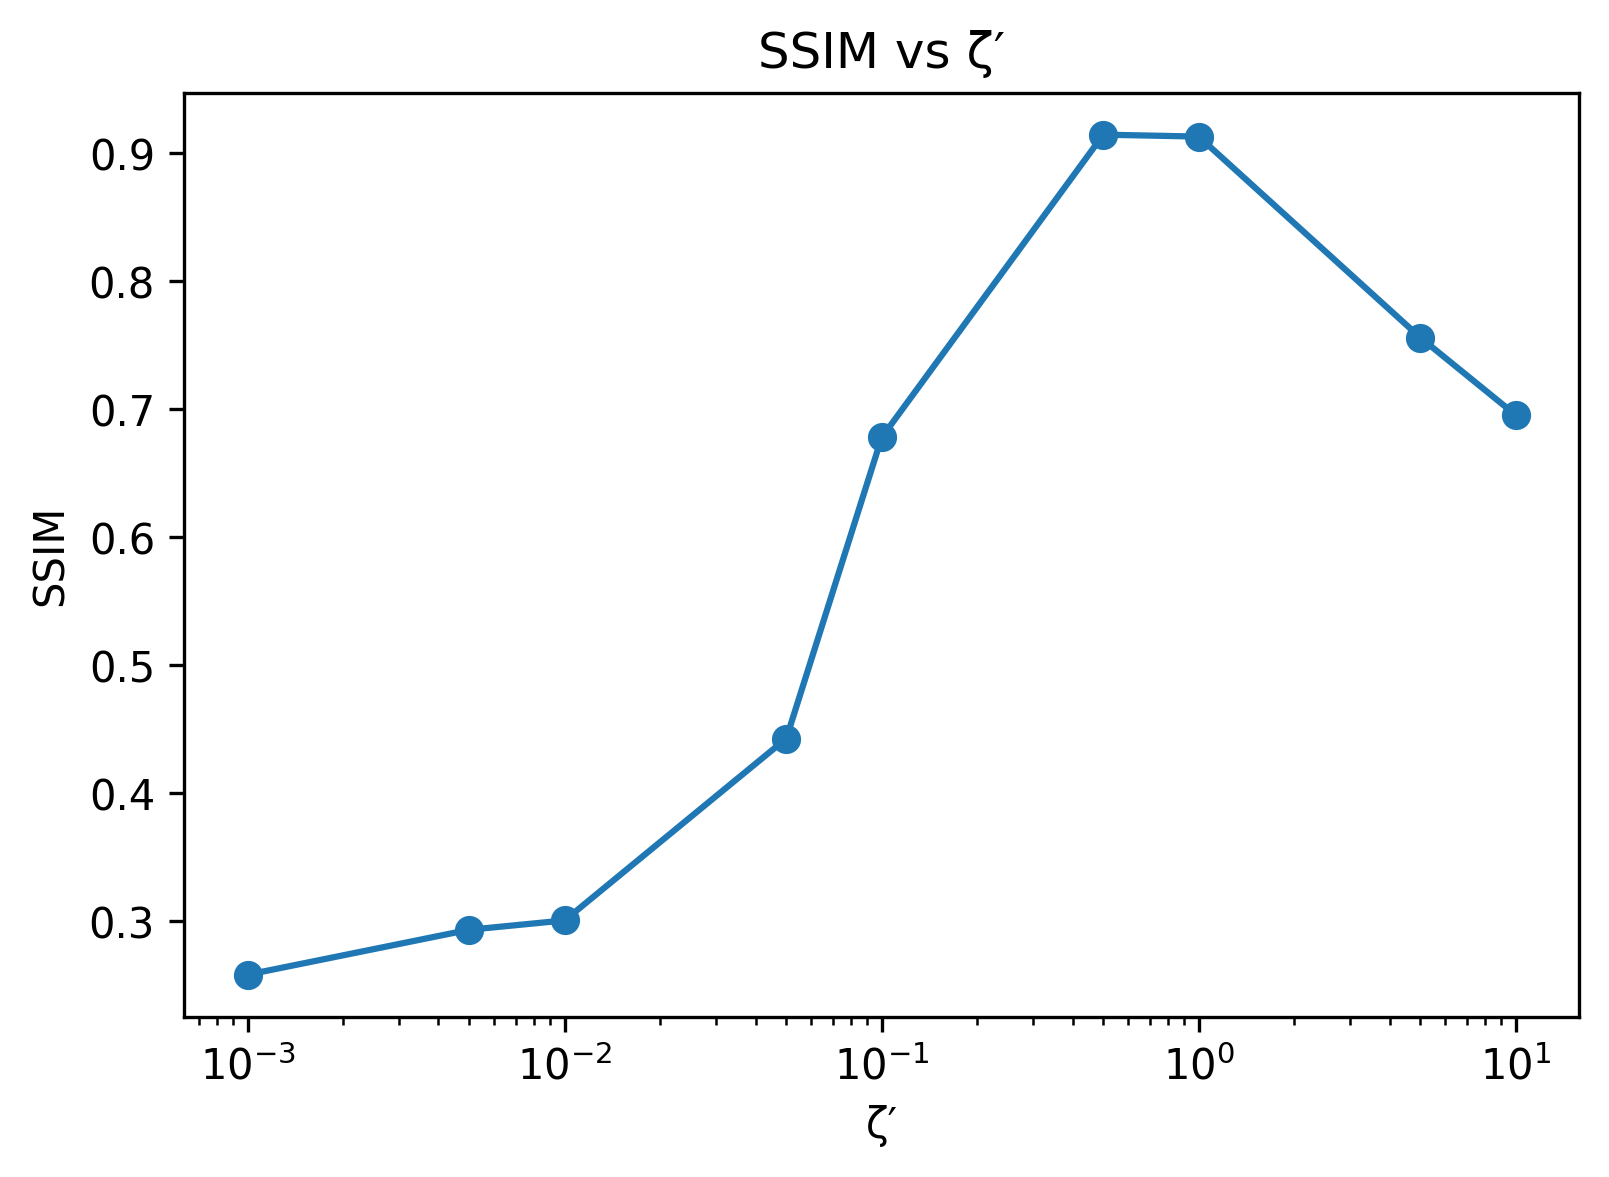
\includegraphics[width=\textwidth]{DPS_VESDE/MNIST/Gauss/SSIM_Gaussian_dps.png}
        \caption{Gaussian SSIM}
        \label{fig:pssim_gauss}
    \end{subfigure}
    \caption{PSNR and SSIM for different $\zeta'$ for Gaussian}
\end{figure}

\subsection{Inpainting}
\begin{figure}[H]
    \centering
    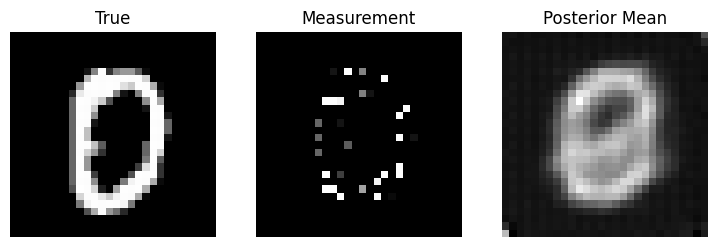
\includegraphics[width=0.8\textwidth]{DPS_VESDE/MNIST/Inpainting/Inpainting_posterior_mean_single_digit.png}
    \caption{Clean, Measurement and Posterior Mean}
    \label{fig:inpaint_post_mean}
\end{figure}

\begin{figure}[H]
    \centering
    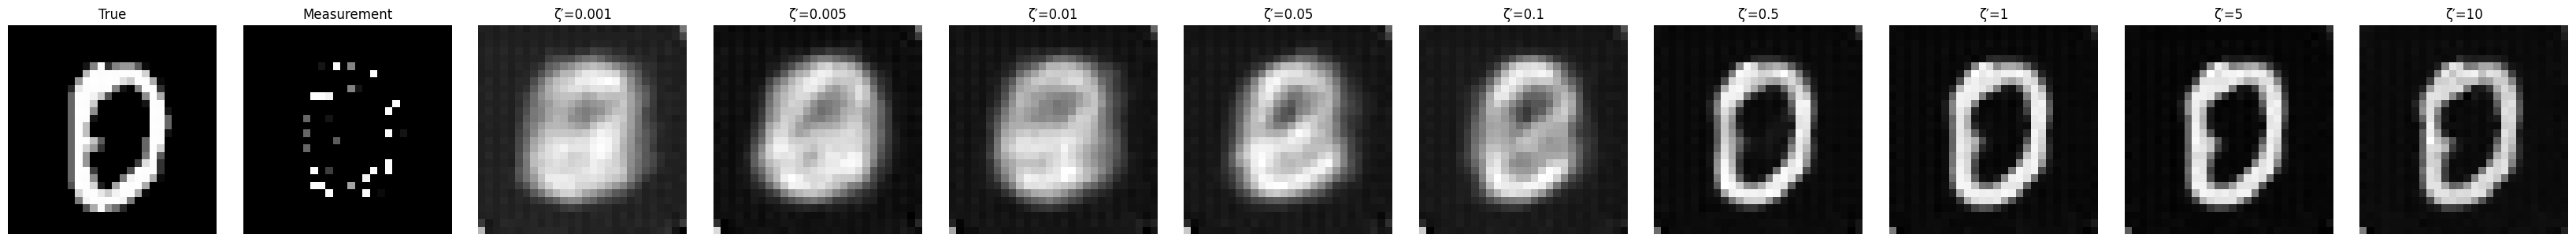
\includegraphics[width=1.0\textwidth]{DPS_VESDE/MNIST/Inpainting/Inpainting_posterior_mean_different_zeta_prime.png}
    \caption{Posterior mean images for different $\zeta'$}
    \label{fig:zeta_prime_inpaint_diff}
\end{figure}

\begin{figure}[htbp]
    \centering
    % First row
    \begin{subfigure}{0.45\textwidth}
        \centering
        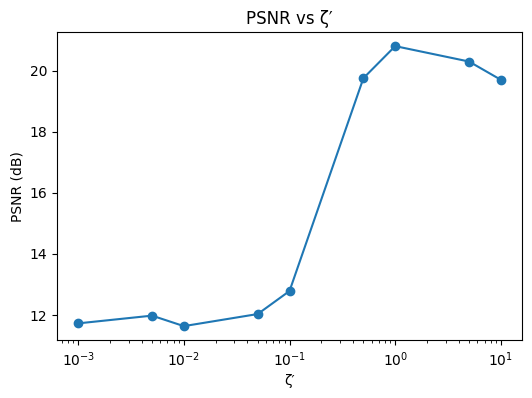
\includegraphics[width=\textwidth]{DPS_VESDE/MNIST/Inpainting/PSNR_Inpainting_dps.png}
        \caption{Inpainting PSNR}
        \label{fig:psnr_inpaint}
    \end{subfigure}
    \hfill
    \begin{subfigure}{0.45\textwidth}
        \centering
        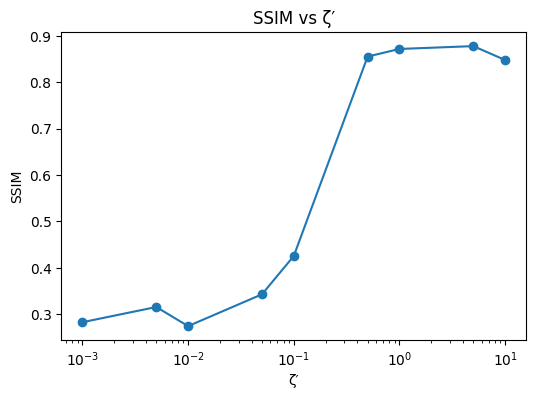
\includegraphics[width=\textwidth]{DPS_VESDE/MNIST/Inpainting/SSIM_Inpainting_dps.png}
        \caption{Inpainting SSIM}
        \label{fig:ssim_inpaint}
    \end{subfigure}
    \caption{PSNR and SSIM for different $\zeta'$ for Inpainting}
\end{figure}

\begin{table}[H]
    \centering
    \caption{PSNR and SSIM for different values of $\zeta'$ under Gaussian and inpainting settings.}
    \label{tab:zeta_comparison}
    \begin{tabular}{c|cc|cc}
        \hline
        \multirow{2}{*}{$\boldsymbol{\zeta'}$}
        & \multicolumn{2}{c|}{\textbf{Gaussian}}
        & \multicolumn{2}{c}{\textbf{Inpainting}} \\
        & \textbf{PSNR (dB)} & \textbf{SSIM}
        & \textbf{PSNR (dB)} & \textbf{SSIM} \\
        \hline
        $0.001$ & 11.69 & 0.2826 & 11.72 & 0.2828 \\
        $0.005$ & 11.61 & 0.2861 & 11.97 & 0.3156 \\
        $0.01$  & 11.77 & 0.2893 & 11.63 & 0.2744 \\
        $0.05$  & 13.37 & 0.4660 & 12.03 & 0.3429 \\
        $0.1$   & 15.84 & 0.6724 & 12.78 & 0.4255 \\
        $0.5$   & 23.83 & 0.9162 & 19.75 & 0.8553 \\
        $1$     & 23.93 & 0.9109 & 20.80 & 0.8717 \\
        $5$     & 17.57 & 0.7583 & 20.30 & 0.8778 \\
        $10$    & 14.66 & 0.6957 & 19.70 & 0.8478 \\
        \hline
    \end{tabular}
\end{table}

\chapter{KSD Framework on Diffusion Posterior Sampling}
\section{Experiments}
Based on all the previous chapters, we now use the KSD framework on the diffusion posterior samples. We now generate noisy images for the fist 10 images of the MNIST even data set using the Gaussian noising. We then use the KSD framework to compute the statistical power of the test for true samples and the DPS samples.

\begin{figure}[htbp]
    \centering
    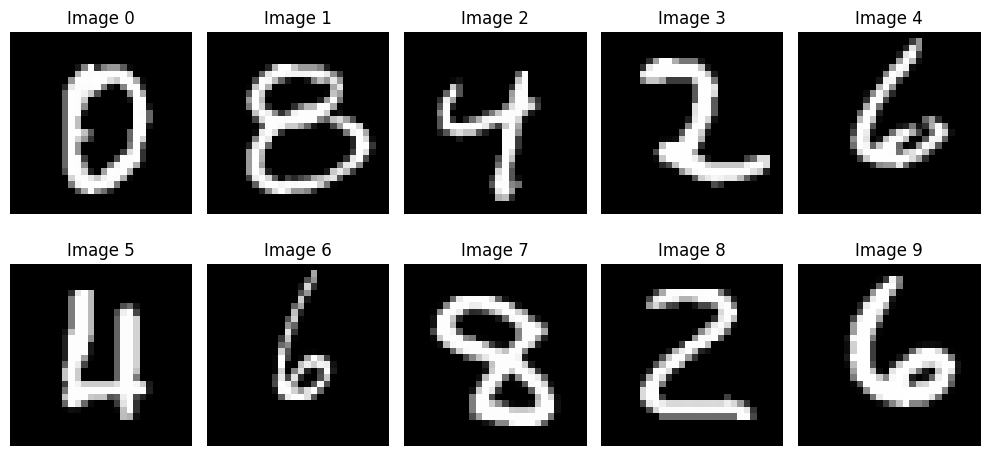
\includegraphics[width=\textwidth]{DPS_VESDE/MNIST/Gauss/clean_10.png}
    \caption{Clean 10 images from MNIST}
    \label{fig:mnist_10_clean}
\end{figure}

\begin{figure}[htbp]
    \centering
    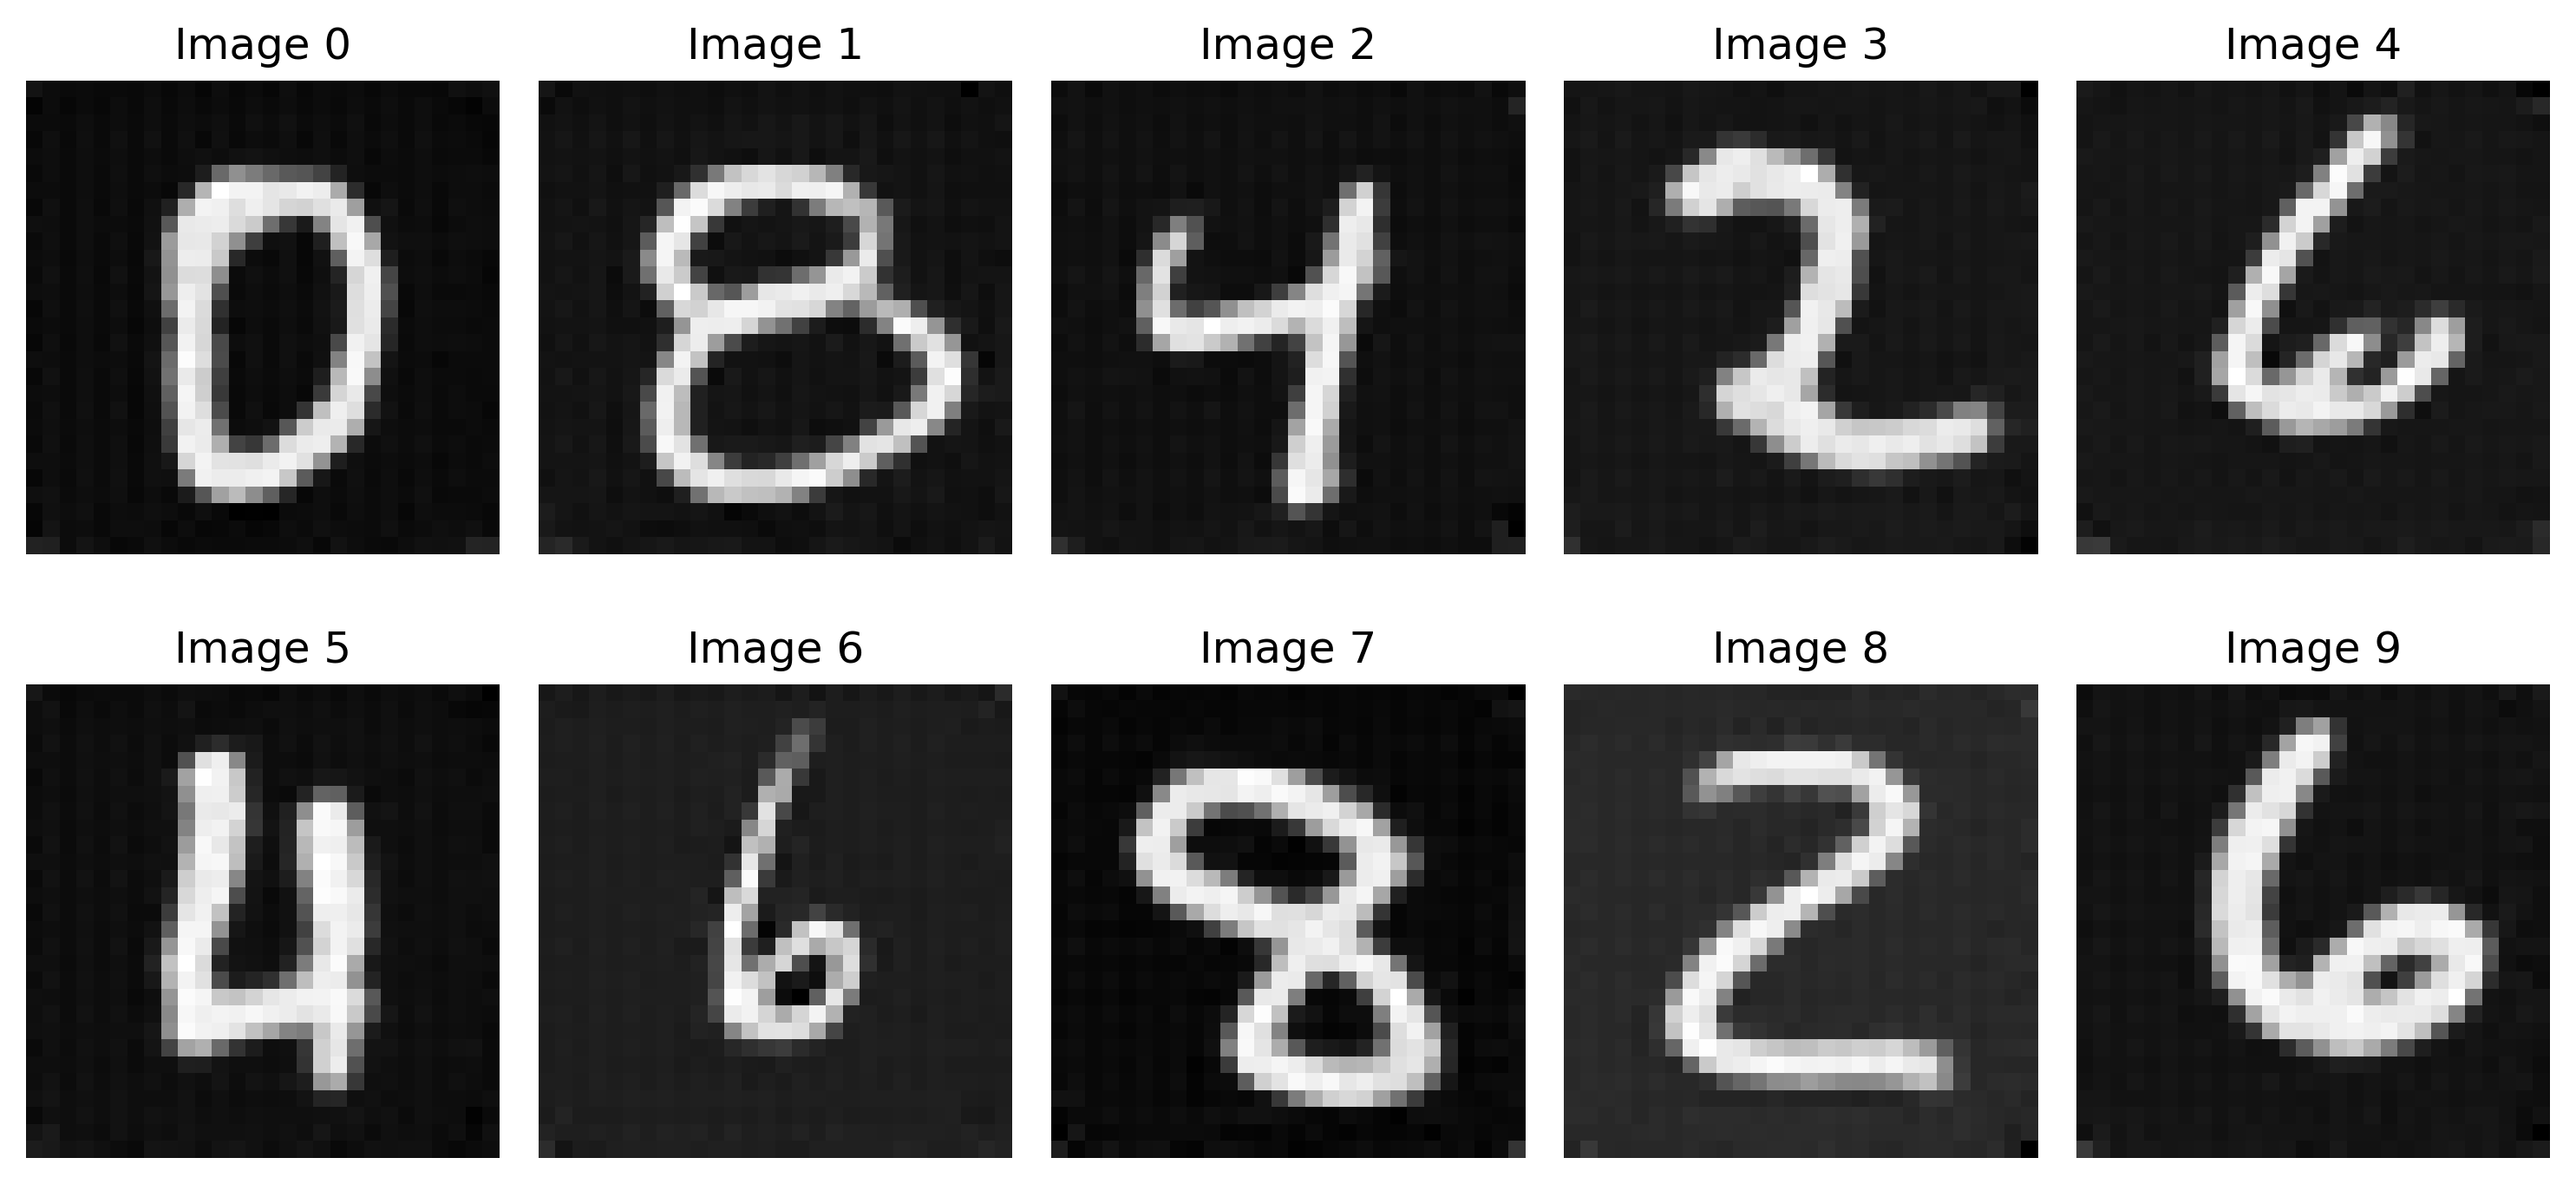
\includegraphics[width=\textwidth]{DPS_VESDE/MNIST/Gauss/Posterior_means_dps_gauss_10.png}
    \caption{Gaussian posterior means 10 images}
    \label{fig:gauss_dps_samples}
\end{figure}

\begin{figure}[H]
    \centering
    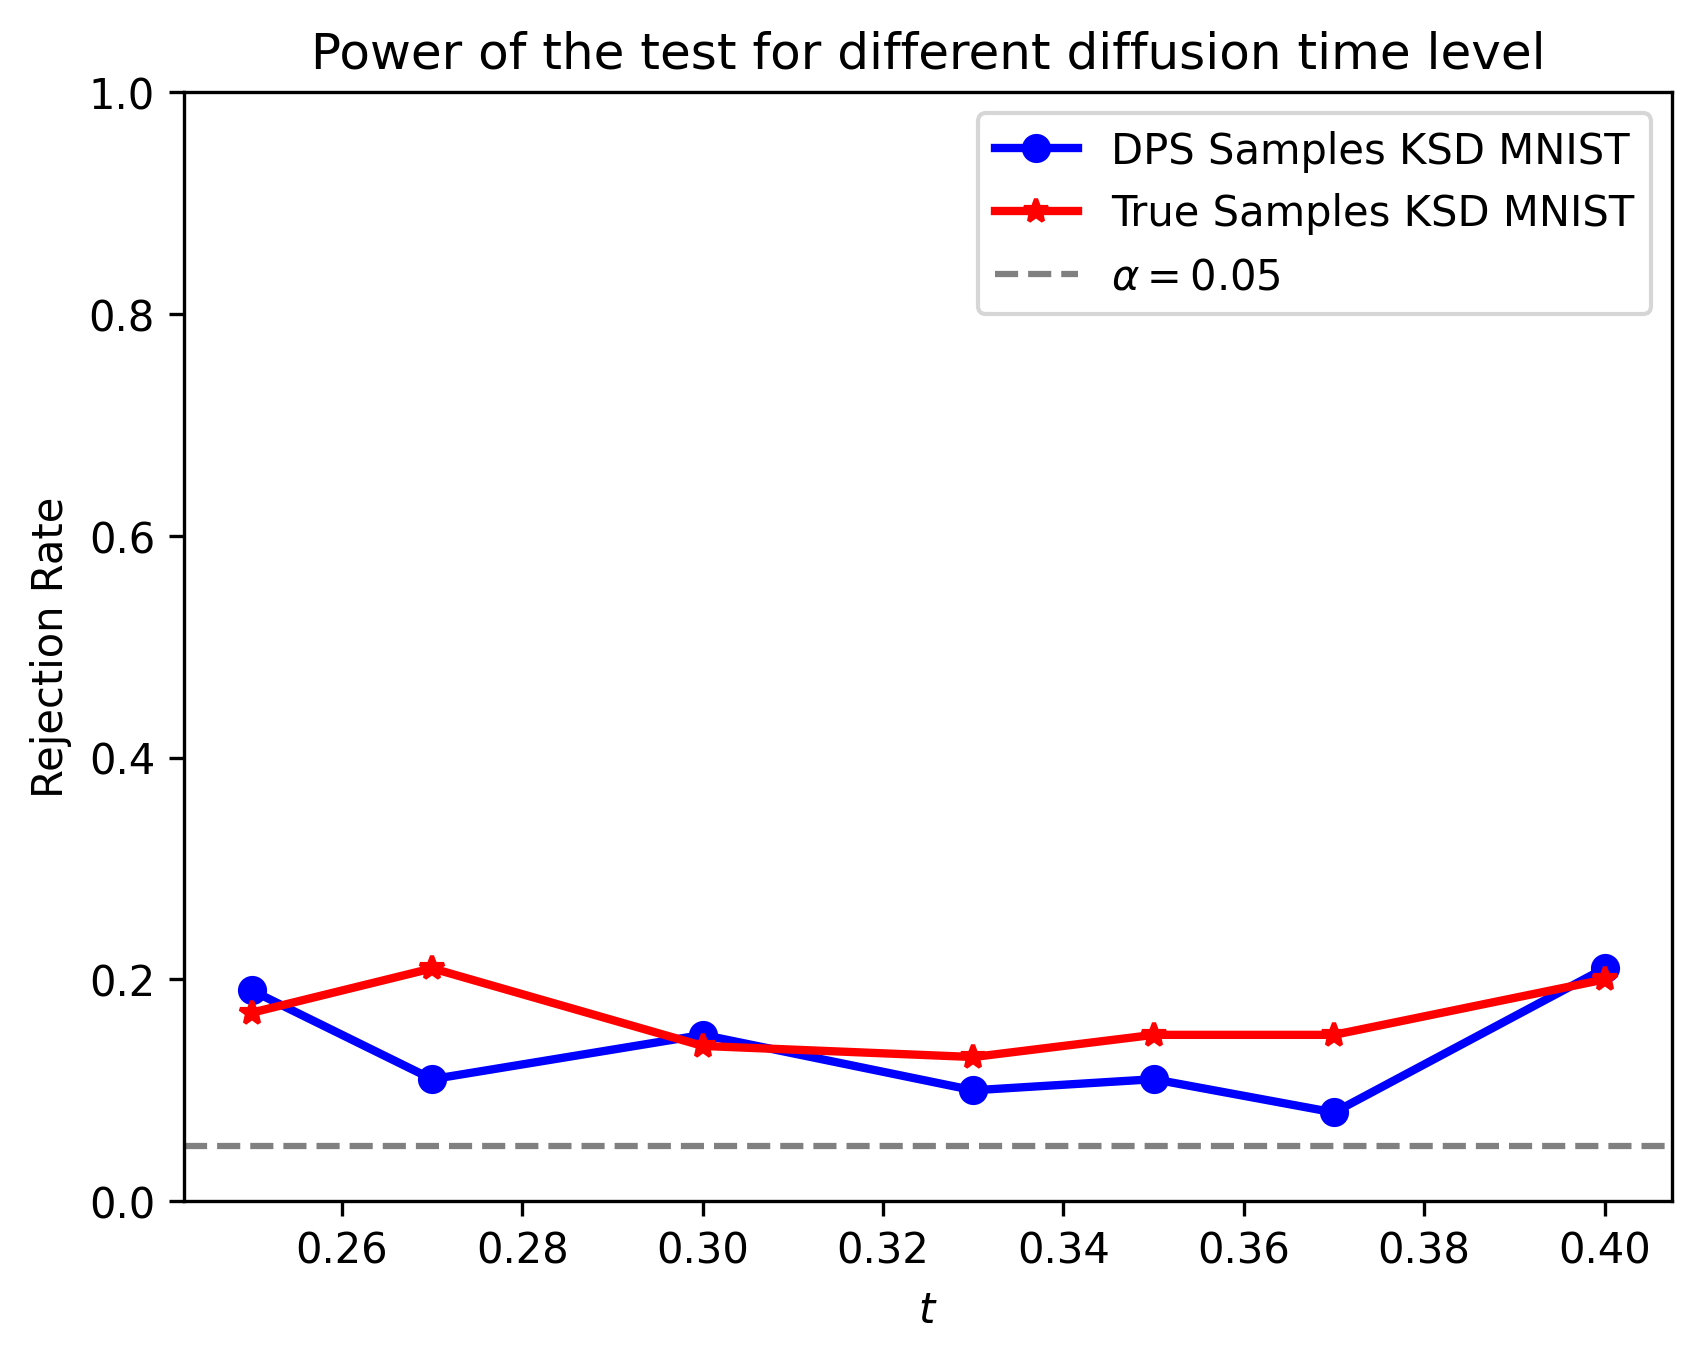
\includegraphics[width=1.0\textwidth]{DPS_VESDE/MNIST/Gauss/ksd_score_dps_gauss_even.png}
    \caption{KSD Power test for DPS Clean samples and True Samples}
    \label{fig:KSD_Test_clean_dps}
\end{figure}

\section{Discussion}
We have applied the KSD framework on the DPS samples and we find that the overall power is similar to bith true and DPS samples, however they are still not close to the desired power level.

\chapter{Conclusion and Future Work}
\section{Conclusion}
We have applied the KSD framework on single mode Gaussian mixture model, and with a trained score network used it on MNIST dataset, which gives us fairly reasonable results. We then used diffusion posterior sampling approach to generate new samples using the same score network and again applied the KSD framework on those DPS samples, which again gave fairly reasonable results.

\vspace{0.3cm}
\noindent
Based on these, we can say that the KSD framework can be applied on multidimensional setups. However it is still computationally expensive, and the power of the statistical tests can still be made to improve.

\vspace{0.3cm}
\section{Future Work}
We can try to use different tests like MMD to get better statistical power. The use of perturbed kernel shows promise for multi-modal setting, however it needs to be applied on image datasets. The use of learned kernel is also helpful which theoretically allows us to increase the power of the test.

\printbibliography[heading=bibintoc,title={References}]
\end{document}